%!TEX root = restart.tex
\RequirePackage{fix-cm}
\documentclass[nospthms,smallextended]{svjour3}       % onecolumn (second format)
\usepackage[T1]{fontenc}
\usepackage[latin9]{inputenc}
\usepackage{listings}
\usepackage{longtable}
\usepackage{float}
\usepackage{wrapfig}
\usepackage{amsmath}
\usepackage{amssymb}
\usepackage{graphicx}
\usepackage{esint}
\usepackage{amsthm}
% \usepackage[sorting=none,url=false, firstinits=true, isbn=false,backend=biber]{biblatex}
% \usepackage[url=false, firstinits=true, isbn=false]{biblatex}
% \addbibresource{AdjointPaper.bib}
% \addbibresource{Remote.bib}


\makeatletter

\providecommand{\tabularnewline}{\\}
\floatstyle{ruled}

%%%%%%%%%%%%%%%%%%%%%%%%%%%%%% LyX specific LaTeX commands.
%% Because html converters don't know tabularnewline
\newtheorem{defn}{Definition}[section]
\newtheorem{prop}{Proposition}[section]
\newtheorem{rem}{Remark}[section]
\newtheorem*{note}{Note}

% \let\oldrem\rem
% \renewcommand{\rem}{\oldrem\normalfont}

% \let\oldnote\note
% \renewcommand{\note}{\oldnote\normalfont}


\newfloat{algorithm}{tbp}{loa}
\providecommand{\algorithmname}{Algorithm}
\floatname{algorithm}{\protect\algorithmname}

\usepackage{fullpage}

\usepackage{subfig}

\makeatother

\DeclareMathOperator{\sgn}{sgn}

\titlerunning{Adjoint-based optimization on conservation law networks}

\authorrunning{Reilly et al}

\institute{$^*$University of California, Berkeley - California, USA, \email{jackdreilly@berkeley.edu}
           \and \at
              $^{\dagger}$Inria Sophia Antipolis - M\'{e}diterran\'{e}e, Sophia Antipolis, France
}

\date{Submitted: \today}

\begin{document}

\title{Adjoint-based Optimization on a Network of Discretized Scalar Conservation
Law PDEs with Applications to Coordinated Ramp Metering}


\author{Jack Reilly$^*$ \and Walid Krichene$^*$ \and Maria Laura Delle Monache$^{\dagger}$ \and Samitha Samaranayake$^*$ \and Paola Goatin$^{\dagger}$ \and Alexandre M. Bayen$^*$}
\maketitle
\newcommand{\R}{\mathbb{R}}


\newtheorem{defn}{Definition}[section]
% \newtheorem{prop}{Proposition}[section]
\newtheorem{rem}{Remark}[section]
\newtheorem*{note}{Note}


\input{adjoint-commands}
This dissertation develops a general, scalable framework for controlling dynamical, networked systems based on mathematical optimization theory, with a strong focus on applications to freeway traffic management. The generality of the framework allows for controllers to consider arbitrary high-level objectives applied to systems with complex, nonlinear dynamics.

The dissertation presents a continuous freeway traffic model and its discretization developed specifically for onramp metering control, the application serving as the motivating example behind the theory developed subsequently. To apply effective control on such systems, a discrete-adjoint-based model-predictive-control (MPC) approach for controlling networked systems of conservation laws is presented, with explicit derivations for ramp metering applications. Linear scalability of the method with respect to network size and time horizon is derived for the discrete adjoint computations. To enable a more asynchronous control architecture, the dissertation presents a distributed optimization algorithm for dynamical, networked systems. The algorithm allows for a physical network to be partitioned into subnetworks that optimize locally and communicate only with adjacent subnetworks to achieve a globally optimal performance. 

Within the context of the \emph{Connected Corridors} project associated with UC Berkeley PATH, the developed theory was implemented in a production-level traffic management and simulation environment. Numerical examples using realistic, calibrated freeway networks are presented alongside the theory to motivate the highly practical aspects of the work. Simulations demonstrate the superiority of the MPC approach over existing methods widely used in practice.

The presented optimization tools are applied to an investigation of the security and vulnerabilities of traffic control systems. The potential impact of a compromise of freeway traffic metering lights is analyzed using MPC and multi-objective optimization tools. Several realizable scenarios that exploit traffic system vulnerability locations are constructed and simulated to illustrate the severity of compromises.

Investigations are made into optimal rerouting strategies while controlling only a subset of network flow. A novel behavioral model is developed to account for the interaction of controllable and uncontrollable agents sharing a single flow network, where latency is a function of total flow. Using static freeway traffic models and communication network models, a framework based on convex optimization techniques is presented for computing rerouting policies, with numerical results.

% effective management of transportation systems is crucial to supporting increasing vehicle demand into the future.

% To improve further the scalability of the adjoint approach and


% A taxonomy of potential attack vectors is developed to classify the cost and controllability of different the different attacks, among other features. 

% Explicit derivations of the approach are given for ramp metering applications along with numerical simulations on realistic freeway models to demonstrate the superiority of the MPC approach over existing methods widely used in practice.

% The splitting technique utilizes an asynchronous extension of the alternating direction method of multipliers algorithm that permits subproblems to apply the previously-developed discrete adjoint method.
\keywords{control of discretized PDEs, network of hyperbolic conservation laws, adjoint based optimization, transportation engineering, ramp metering}
\chapter{Introduction}
\label{sec:introduction}

\section{Motivation}
\label{sec:motivation}

% \todo[inline]{lots of ``systems'' written here}

Modern infrastructure, particularly systems associated with public use such as freeway networks and water supplies, exist within a world with decreasing physical space and resources. For instance, freeways often cannot add additional lanes to accommodate increased demands. Thus, one must rely upon better management systems and control algorithms in order to maximize performance within the limitations of the existing system. These ``smart'' systems make use of sensing instrumentation to estimate real-time conditions and modeling of the underlying physical dynamics to predict and plan for future states.

The focus of this thesis is the development of methods for the advanced modeling and control of such networked dynamical systems. The goal is to provide operational managers with scalable, flexible, and robust algorithms that can leverage the well-instrumented and highly-connected control infrastructure present on modern systems. 

The remainder of this section discusses the \emph{Connected Corridors} project (Section~\ref{sec:connected-corridors}) on \emph{integrated corridor management} (ICM), which served as the context in which this work was conducted, followed by an overview of \emph{model predictive control} (MPC) methods and their suitability in solving some of the main objectives put forth in the \emph{Connected Corridors} project (Section~\ref{sec:model-predictive-control}). The section concludes with a summary of the original contributions presented in this thesis (Section~\ref{sec:contributions}).

\section{Connected Corridors}
\label{sec:connected-corridors}

\emph{Connected-Corridors} is a project funded by the California Department of Transportation with the goal of creating the next generation of traffic management tools~\cite{connected-corridors,miller2010san}. While most current systems consider the freeway networks as independent from the city-street \emph{arterial} road networks, \emph{Connected Corridors} is tasked with creating an integrated approach to traffic management (referred to as ICM) which accounts for their dual performance. The project has demonstrated innovative control and estimation approaches to ICM on macroscopic and microscopic simulation environments (presented in Section~\ref{sec:numerical-results-adjoint}), with the ultimate plan of transferring the knowledge to a physical test-site within California located near the I210 freeway.

The proposed ICM system possesses the following capabilities.

\begin{itemize}
	\item \textbf{Estimation}: Operators have access to a real-time estimation of the traffic state along the major freeways and adjacent arterials~\cite{work2010traffic,Jacqueta,eisenman2006number}.
	\item \textbf{Simulation}: Well-calibrated and efficient traffic models allow operators to simulate many different future traffic conditions~\cite{Muralidharan2009b,dervisoglu2014macroscopic,Hunter}.
	\item \textbf{Control}: Traffic signal and message sign plans are computed online for a variety of specialized objectives and serve as an optimized decision support tool~\cite{Reilly2013b,Reilly2014b}.
\end{itemize}

Control schemes implemented by the system include coordinated traffic light metering plans on freeway onramps (commonly referred as ramp metering, see Section~\ref{sec:continous-and-discrete-traffic-model-for-ramp-metering}) and traffic flow diversion around incidents via changeable message signs~\cite{Samaranayake2014}. 

\begin{figure}[htbp]
	\centering
	\includegraphics[width=0.7\textwidth]{diagrams/f2}
	\caption[\emph{Connected Corridors} control system architecture.]{The freeway state estimation, prediction and calibration submodules enable an MPC-based framework that computes coordinated, predictive decision-support strategies for numerous applications. Limited customization is required to extend the adjoint-based MPC controller to specific objectives or actuation types.}
	\label{fig:decision-support}
\end{figure}

To satisfy the above requirements, \emph{Connected Corridors} focuses on a number of submodules which are developed independently, but composed in a variety of ways to create high-level, comprehensive support tools. Figure~\ref{fig:decision-support} shows several of the developed submodules and how they can be composed to create an MPC controller (explained in Section~\ref{sec:model-predictive-control}). Subsequently, the controller submodule is leveraged by a number of actuation strategies which have similar architectural requirements. For instance, both ramp metering and dynamic rerouting require real-time estimation and a calibrated freeway model to compute effective control strategies. Via submodule composition, much of the technology can be reused between the applications. This work contains the theory and implementation of constructing such controller submodules which efficiently exploit the structure of freeway networks.

\section{Model Predictive Control}
\label{sec:model-predictive-control}

Central to the \emph{Connected Corridors} approach of freeway traffic decision support is the concept of \emph{model predictive control} (MPC)~\cite{Muralidharana,Donoghue2013Splitting,Frejo2011}. Generally speaking, MPC schemes successively compute a control policy which maximizes the performance, according to a provided criteria, of the system over the immediate future, where this work assumes the future to be of finite duration. The policy generated from the MPC scheme is recomputed as frequently as the real-time state estimation and computation times permit. Thus, associated with an MPC problem are two time periods: the \emph{update time} representing how often the MPC policy is recomputed online, and the \emph{time horizon} representing how far into the future for which the MPC policy will account. A more detailed treatment of MPC schemes is given in Section~\ref{sec:model-predictive-control-overview-adjoint-section}.

The requirements of an online MPC controller for a traffic system are depicted in Figure~\ref{fig:decision-support}. At the base of the method is a mathematical model of the physical system, referred to as the \emph{forward system}. These models often require calibration using historical sensor measurements to set the model parameters. To fully specify the simulation, an \emph{initial condition} is specified (i.e. estimation), as well as the \emph{boundary conditions} at the exteriors of the system over the entire time horizon of the MPC problem (i.e. prediction). All these requirements are satisfied by components within the \emph{Connected Corridors} system~\cite{Muralidharan2009b,dervisoglu2014macroscopic,work2010traffic}, making MPC control a natural fit for research and development in the project.

The focus of this thesis is the efficient and flexible design of MPC optimization techniques and their applications to freeway control systems. At the heart of the developed approach is the \emph{discrete adjoint} method for gradient computations within first-order gradient descent methods (Chapter~\ref{chapter:adjoint}). The efficiency of the developed method enables \emph{online} application of MPC to the control of large freeway networks (on the order of tens of miles) with frequent recomputations (on the order of one minute) to ``close the loop'' with real-time measurements.

In addition to the well-established ramp metering control infrastructure, the emergence of smartphones and connected vehicles and crowd-sourcing data collection~\cite{Reilly2013,Ervasti2011,dashti2013evaluating} has made mass rerouting strategies a new, viable form of control. This thesis showcases this potential by including an investigation of rerouting strategies for a subset of flow on networks. Inspired by the increasing penetration of navigation devices in vehicles (e.g. dedicated units, smartphone applications), a single navigation provider may advise a signification portion of the total flow on some networks, thus potentially affecting traffic conditions based on their advice. This potential can be harnessed to reduce the inefficiencies of \emph{selfish routing}~\cite{roughgarden2002bad,krichenetac} and drive network behavior towards \emph{socially optimal} conditions.

\section{Contributions}
\label{sec:contributions}

This thesis contains the following contributions to the problem of optimal control of networked dynamical systems, applied to the field of traffic control.

\begin{itemize}
	\item \textbf{A novel continuous freeway traffic model suitable for finite-horizon optimal control problems}~\cite{delle2014pde,Reilly2013b}.
	\begin{itemize}
		\item The model represents an extension of the networked \emph{Lighthill-Richards-Whitham} (LWR) PDE traffic model~\cite{lighthill1955kinematic,richards1956shock} proposed in~\cite{garavello2006traffic}, where onramps are modeled as ODE buffers to guarantee \emph{strong} boundary conditions and flow conservation at the network boundaries.
		\item A discretized version of the continuous model is derived for optimal control application using Godunov's method~\cite{godunov1959,lebacque1996godunov}.
	\end{itemize}
	\item \textbf{A method for optimal control of networked conservation law systems based on discrete adjoint calculations}~\cite{Reilly2013b,Samaranayake2014}.
	\begin{itemize}
		\item This work develops a framework for converting a continuous time and space control problem on a physical network, where edges behave according to a conservation law, into a discrete, finite-horizon optimal control problem using Godunov discretization.
		\item The application of the discrete adjoint method~\cite{Giles2000,Duffy2009,Apice2010Modeling,Gugat2005} to compute gradients for the above problem is presented, with an analysis of the linear scalability of the approach in discrete time and discrete space for sparse network structures.
		\item An explicit formulation of the discrete adjoint method is given for the application of coordinated ramp metering control~\cite{Papageorgiou1991,Frejo2011,Kotsialos2004,gomes2006optimal} for freeway networks.
		\item Simulations of MPC on a macroscopic model of the I15 South Freeway in San Diego, California demonstrate the practical nature and the robustness to measurement noise of the research.
	\end{itemize}
	\item \textbf{A decentralized algorithm and control infrastructure for networked dynamical systems}~\cite{Reilly2014b}.
	\begin{itemize}
		\item This thesis presents a new distributed optimization method based on the \emph{alternating directions methods of multipliers} (ADMM)~\cite{Boyd2010a,gabay1976dual,mota2012distributed} algorithm for solving  optimal control problems over subnetworks in parallel. The splitting method is done in such a way to only require communication between physically-neighboring subnetworks.
		\item Differing from similar work where subsystems only share control variables~\cite{mota2012distributed,camponogara2009distributed}, the presented method allows for subsystems to share both control \emph{and state} variables, an assumption necessary for the distributed control of traffic networks and hydrological systems.
		\item A discrete adjoint formulation is presented for efficient solution of subsystems with coupled control and state variables.
		\item An implementation of a distributed ramp metering and variable speed limit controller is simulated on a realistic macroscopic freeway network, demonstrating advantages over other proposed communicative controllers.
	\end{itemize}
	\item \textbf{An analysis of the security of traffic control systems and coordinated ramp metering attacks}~\cite{Reilly2014c}.
	\begin{itemize}
		\item A classification of traffic system vulnerability locations is constructed across such categories as cost of attack, effectiveness, and directness of control.
		\item A novel analysis of the potential damage and impact of coordinated ramp metering attacks is conducted using adjoint-based optimal control and multi-objective optimization tools.
		\item Illustrative attack scenarios are constructed and numerically investigated on realistic freeway networks. A web-based coordinated ramp metering attack tool was created to implement the interactive optimization approaches presented in the work~\cite{smartroadswebsite}.
	\end{itemize}
	\item \textbf{A framework for rerouting a subset of vehicles on freeway networks}.
	\begin{itemize}
		\item As opposed to standard system-optimal routing problems~\cite{ziliaskopoulos2000linear,Kelly} where all flow is controllable, we construct a network-flow optimization problem which allows one to specify a \emph{compliance rate} of cooperative vehicles. The proposed model captures the delays induced by the noncompliant vehicles.
		\item To account for the possibility of noncompliant drivers adapting to the new flow conditions, we propose a behavioral model, referred to as \emph{bounded tolerance}, which assumes that noncompliant drivers have bounded rationality and will only switch routes under significant increases in delay.
		\item Numerical examples for communication networks and freeway systems demonstrate the effectiveness of the method.  
	\end{itemize}
\end{itemize}

\section{Organization}
\label{sec:organization}

The rest of the article is organized as follows.

Chapter~\ref{chapter:freeway-network-model} presents the continuous and discrete freeway models which serves as the running application of the theory presented subsequently.  After covering preliminaries on networked PDE systems, the derivation of and motivation behind the model are given.

Chapter~\ref{chapter:adjoint} presents the discrete adjoint approach to optimal control of networked conservation laws. Presented first is a general overview of the discrete adjoint method, followed by its specific instantiation for discretized physical network systems. The application to coordinated ramp metering is then presented with numerical examples. The chapter concludes with the distributed, asynchronous formulation of the adjoint optimal control method via subnetwork splitting.

Chapter~\ref{chapter:security} presents a study of traffic control systems and their vulnerabilities. After defining the specific control system under consideration and its security weaknesses, the work gives an in-depth study of coordinated ramp metering attacks.

Finally, we conclude with a overview of the work presented, as well as directions for future research.

The material presented in Chapters~\ref{chapter:freeway-network-model} and~\ref{chapter:adjoint} was done collaboratively as part of the \emph{Optimal Reroute Strategies for Traffic Management} (ORESTE) project between UC Berkeley and INRIA research institute in Sophia-Antipolis, France. Chapter~\ref{chapter:security} also contains research stemming from collaborations with Sebastien Martin and Mathias Payer. Chapters~\ref{sec:distributed_optimization_of_coupled_dynamical_systems} and~\ref{chapter:le} contains research conducted independently.
We consider the non-linear conservation equation of the form:
\begin{equation}
\partial_t\rho\left(t,x\right)+\partial_x f\left(\rho\left(t,x\right)\right)=0 \quad (t,x) \in \R^+ \times \R\label{eq:cons}
\end{equation}
where $\rho=\rho(t,x) \in \; \R^+$ is the scalar conserved quantity and $f:\R^+\rightarrow \R^+$ is a Lipschitz continuous flux function~\cite{Bressan2000Hyperbolic}. Throughout the article we suppose that $f$ is a concave function. \\
The Cauchy problem to solve is then 
\begin{equation}
	\label{eq:CP}
		\left\{
		\begin{array}{ll}
		\partial_t \rho+ \partial_x f(\rho) =0, & (t,x)\in\R^+\times \R,\\
		\rho(0,x)=\initstate(x), & x \in \R\\
		\end{array}
		\right.
\end{equation}
where $\initstate(x)$ is the initial condition.
It can be shown that there exists a unique weak entropy solution for the Cauchy problem\eqref{eq:CP},  as described in Definition \ref{def:weak-sol}. 
\begin{defn}\label{def:weak-sol}
A function $\rho \in \; \mathcal{C}^0(\R^+; \mathbf{L}^1_{loc}\cap \mathbf{BV})$ is an admissible solution to \eqref{eq:CP} if $\rho$ satisfies the Kru\v{z}hkov entropy condition \cite{Kruzhkov} on $(\R^+\times\R)$, i.e.,for every $k\in \R$ and for all $\varphi \in \mathcal{C}^1_c(\R^2;\R^+),$
\begin{eqnarray}
\label{eq:kruzhkov}
	&\int_{\R^+}\int_{\R}(\modulo{\rho -k}  \partial_t \varphi + \sgn{(\rho-k }) (f(\rho)-f(k))\partial_x\varphi)dxdt& \nonumber\\
	 &+\int_{\R}\modulo{\initstate-k}\varphi(0,x)dx\geq 0.&
\end{eqnarray} 
\end{defn}
For further details regarding the theory of hyperbolic conservation laws we refer the reader to~\cite{garavello2006traffic,Evans1998}.

\paragraph*{Networks}

A network of hyperbolic conservation laws such as~(\ref{eq:cons})
is defined as a set of $\nlinks$ links $\links=\intrange 1{\nlinks}$,
with junctions $\jns$. Each junction $\jn\in\jns$ is defined
as the union of  two non-empty sets: the set of $\ninc_{\jn}$ incoming links $\Inc\left(\jn\right)=\tuple{\jlink{\jn}1}{\jlink{\jn}{\ninc_{\jn}}}\subset\links$
and the set of $\nout_{\jn}$ outgoing links $\Out\left(\jn\right)=\tuple{\jlink{\jn}{\ninc_{\jn}+1}}{\jlink{\jn}{\ninc_{\jn}+\nout_{\jn}}}\subset\links$.
Each link $\link\in\links$ has an associated upstream junction $\jup{\link}\in\jns$
and downstream junction $\jdown{\link}\in\jns$, and has an associated
spatial domain $\left(0,L_{\link}\right)$ over which the evolution
of the state on link $\link$, $\rho_{\link}\left(t,x\right)$, solves
the Cauchy problem:

\begin{equation}
\begin{cases}
\left(\rho_{\link}\right)_{t}+f\left(\rho_{\link}\right)_{x} & =0\\
\rho_{\link}\left(0,x\right) & =\initstate_{\link}\left(x\right)
\end{cases}\label{eq:cauchy-i}
\end{equation}
where $\initstate_{\link}\in BV\cap L_{\text{loc}}^{1}\left(L_i;\mathbb{R}\right)$
is the initial condition on link $\link$. For simplicity of notation,
this section considers a single junction $\jn\in\jns$ with $\Inc\left(\jn\right)=\left(1,\ldots,\ninc\right)$
and $\Out\left(\jn\right)=\left(\ninc+1,\ldots,\ninc+\nout\right)$.
\begin{rem}
There is redundancy in the labeling of the junctions, if link
$i$ is directly upstream of link $j$, then we have $\jdown{\link}=\jup j$.
See Fig.~\ref{fig:Space-discretization-for}.
\end{rem}
While the dynamics on each link $\rho_{\link}\left(t,x\right)$ is
determined by~(\ref{eq:cauchy-i}), the dynamics at junctions
still needs to be defined.



\begin{defn}
\label{def:Riemann-Problem}Riemann Problem.

A Riemann problem is a Cauchy problem~\eqref{eq:CP} with a piecewise-constant initial datum (called the Riemann datum):

\[
\initstate(x)=\begin{cases}
\rho_{-} & x<0\\
\rho_{+} & x\ge 0
\end{cases}
\]
%with one point of discontinuity, $x=\bar{x}$. Without loss of generality,
%we may take $\bar{x}=0$.
\end{defn}
%It can be shown that the $\rho$ solution generated from the Riemann
%data $\left(\rho_{-};\rho_{+}\right)$ has a constant value along
%lines of constant $\frac{x}{t}$. 
We denote the corresponding self-similar entropy weak solutions by $\ss{\frac{x}{t}}{\rho_{-}}{\rho_{+}}$.





\begin{defn}
Riemann problem at junctions. 

A Riemann problem at $\jn$ is a Cauchy problem corresponding to an initial datum $\tuple{\initstate_{1}}{\initstate_{\ninc+\nout}}\in\mathbb{R}^{\ninc+\nout}$ which is constant on each link $\link.$

%Let all links $\link$ have a constant initial profile $\rho_{\link}\left(0,x\right)=\initstate_{\link}\in\mathbb{R}$
%(called the Riemann data) with incoming links having a spatial domain
%$\left(-\infty,0\right)$ and outgoing links having a spatial domain
%$\left(0,\infty\right)$. The solution of $\rho_{\link}\left(x,t\right)$
%for all links $\link\in\Inc\left(\jn\right)\cup\Out\left(\jn\right)$
%and $t\ge0$ is defined as the solution to the Riemann problem at
%junction $J$ with initial data $\tuple{\initstate_{1}}{\initstate_{\ninc+\nout}}\in\mathbb{R}^{\ninc+\nout}$.
\end{defn}
\begin{defn}
A Riemann solver is a map that assigns a solution to each Riemann initial data. For each junction $\jn$ it is a function

\begin{eqnarray*}
\RS: & \mathbb{R}^{m+n} & \rightarrow\mathbb{R}^{m+n}\\
 & \tuple{\initstate_{1}}{\initstate_{\ninc+\nout}} & \mapsto\RS\tuple{\initstate_{1}}{\initstate_{\ninc+\nout}}=\tuple{\trace{\rho}_{1}}{\trace{\rho}_{\ninc+\nout}}
\end{eqnarray*}
where $\trace{\rho}_{\link}$ provides the trace for link $\link$
at the junction for all time $t\ge0$.

\end{defn}
For a link $i\in\Inc\left(\jn\right)$,
the solution $\rho_{i}\left(t,x\right)$ over its spatial domain
$x<0$ is given by the solution to the following Riemann problem:

\begin{equation}
\begin{cases}
\left(\rho_{\link}\right)_{t}+f\left(\rho_{\link}\right)_{x} & =0\\
\rho_{\link}\left(0,x\right) & =\begin{cases}
\initstate_{\link} & x<0\\
\trace{\rho}_{\link} & x\ge0,
\end{cases}
\end{cases}\label{eq:riemann-problem}
\end{equation}

The Riemann problem for an outgoing link is defined similarly, with
the exception that $\rho_{\link}\left(0,x>0\right)=\initstate_{\link}$
and $\rho_{\link}\left(0,x\le0\right)=\trace{\rho}_{\link}$. 

Fig.~\ref{fig:Solution-of-boundary}
gives a depiction of Riemann solution at the junction.%

\begin{figure}
\begin{centering}
\includegraphics[width=0.5\columnwidth]{presentation/figs-gen/junctions-riemann-rs} 
\par\end{centering}

\caption{Solution of boundary conditions at junction. The boundary conditions
$\tuple{\trace{\rho}_{1}}{\trace{\rho}_{5}}$ are produced by applying
the Riemann solver to the initial conditions, $\tuple{\initstate_{1}}{\initstate_{5}}$.\label{fig:Solution-of-boundary}}
\end{figure}


Note that the following properties for the Riemann Solver holds:
\begin{itemize}
\item All waves produced from the solution to Riemann problems on all links,
generated by the boundary conditions at a junction, must emanate out
from the junction. Moreover, the solution to the Riemann problem
on an incoming link must produce waves with negative speeds, while
the solution on an outgoing link must produce waves with positive
speed. 
\item The sum of all incoming fluxes must equal the sum of all outgoing
fluxes: 
\[
\sum_{i\in\Inc\left(\jn\right)}f\left(\trace{\rho}_{\link}\right)=\sum_{j\in\Out\left(\jn\right)}f\left(\trace{\rho}_{j}\right).
\]
This condition guarantees mass conservation at junctions.
\item The Riemann solver must produce self-similar solutions, i.e. 
\[
\RS\left(\RS\tuple{\initstate_{1}}{\initstate_{\ninc+\nout}}\right)=\RS\tuple{\initstate_{1}}{\initstate_{\ninc+\nout}}=\tuple{\trace{\rho}_{1}}{\trace{\rho}_{\ninc+\nout}}
\]
\end{itemize}

The justification for these conditions can be found in~\cite{garavello2006traffic}.

The above conditions are not always sufficient to guarantee a unique Riemann solver. Additional conditions are added for specific applications to achieve uniqueness, chosen to model physical phenomena at junctions. In Section~\ref{sec:Applications-to-Optimal}, we detail the additional conditions added to the ramp-metering solver which enforce flux maximization along the freeway mainline sections and specify a merging priority model for vehicles entering from the onramps.


\subsection{Godunov Discretization\label{sub:Godunov-Discretization}}

In order to find approximate solutions we use the classical Godunov scheme~\cite{godunov1959}. We use the following notation: $x_{j+\frac{1}{2}}$ are the cell interfaces and   $t^{\tind}=k\Delta t$ the time with $\tind\in\mathbb{N}$ and $\xind\in\mathbb{Z}$. $x_{\xind}$ is the center of the cell, $\Delta x=x_{j+\frac{1}{2}}-x_{j-\frac{1}{2}}$ the cell width, and $\Delta t$ is the time step. 
\paragraph{Godunov scheme for a single link.}

The Godunov scheme is based on the solutions of exact Riemann problems. The main idea of this method is to approximate the initial datum by a piecewise constant function, then the corresponding Riemann problems are solved exactly and a global solution is found by piecing them together. Finally one takes the mean on the cell and proceed by iteration. Given $\rho(t,x),$ the cell average of $\rho$ at time $t^{\tind}$ in the cell $C_{\xind}=]x_{j-\frac{1}{2}},x_{j+\frac{1}{2}}]$ is given by 
\begin{equation}
\discrete{\xind}{\tind}=\dfrac{1}{\Delta x}\int_{\xdis{\xind-\frac{1}{2}}}^{\xdis{\xind+\frac{1}{2}}}\dvar(t^{k},x)dx.\label{eq:godproj}
\end{equation}
Then we proceed as follows:
\begin{enumerate}
	\item We solve the Riemann problem at each cell interface $x_{j+\frac{1}{2}}$ with initial data $(\dvar^{\tind}_{\xind},\dvar^{\tind}_{\xind+1}).$
	\item Compute the cell average at time $t^{\tind +1}$ in each computational cell and obtain $\dvar^{\tind +1}_{\xind}.$ 
\end{enumerate}

We remark that waves in two neighbouring cells do not intersect before $\Delta t$ if the following Courant\textendash{}Friedrichs\textendash{}Lewy (CFL) condition holds, $\lambda^{\max}\le\frac{\Delta x}{\Delta t}$, where $\lambda^{\max}=\underset{a}{\max}|f'\left(a\right)|$ is the maximum wave speed of the Riemann solution at the interfaces.\\
Godunov scheme can be expressed as follows:
\begin{equation}
\discrete{\xind}{\tind+1}=\discrete{\xind}{\tind}-\frac{\Delta t}{\Delta x}(\god(\discrete{\xind}{\tind},\discrete{\xind+1}{\tind})-\god(\discrete{\xind-1}{\tind},\discrete{\xind}{\tind})),\label{eq:godscheme}
\end{equation}
where $g^{G}$ is the Godunov numerical flux given by

\begin{eqnarray*}
\god: & \mathbb{R}\times\mathbb{R} & \rightarrow\mathbb{R}\\
 & \left(\discrete{\xind}{},\discrete{\xind+1}{}\right) & \mapsto\god\left(\discrete{\xind}{},\discrete{\xind+1}{}\right)=f(W_{R}(0;\discrete{\xind}{},\discrete{\xind+1}{})).
\end{eqnarray*}

where $W_{R}$ is as defined in Definition~\ref{def:Riemann-Problem}.


%To approximate a hyperbolic PDE of the form in~(\ref{eq:cons-smooth})
%with a discretization in both space and time, we use Godunov's scheme~\cite{godunov1959}.
%Given an initial condition that is piecewise-constant, Godunov's scheme
%gives a procedure to advance the system one time-step forward. Under
%suitable stability conditions, this process can be repeated \emph{ad
%infinum }by applying the scheme to the new condition generated from
%the previous time-step.

%We define a numerical grid using the following notations 
%\begin{itemize}
%\item $\Delta x$ is the fixed space grid size,
%\item $\Delta t$ is the fixed time grid size, chosen with respect to the Courant\textendash{}Friedrichs\textendash{}Lewy (CFL) condition%
%\footnote{This method can be generalized to non-uniform grid sizes, but is chosen
%to be uniform to simplify notation%
%}, 
%\item $(t^{\tind},\xdis{\xind})=(k\Delta t,\xind\Delta x)$ for $\tind\in\mathbb{N}$
%and $\xind\in\mathbb{Z}$ grid points%
%\footnote{The CFL condition, $\lambda^{\max}\le\frac{\Delta x}{\Delta t}$,
%guarantees that the waves in two neighboring cells do not interact
%at the cell boundaries before $\Delta t$. Above $\lambda^{\max}=\underset{a}{\max}|f'\left(a\right)|$
%is the maximum absolute wave speed. We assume henceforth that this
%condition always holds for the chosen step sizes.%
%}. For a link $\link\in\links$ with space domain $\left(0,\length_{\link}\right)$,
%$\xind$ takes values in $\intrange 0{\length_{\link}^{\Delta}}$.
%\end{itemize}
%For a function $\dvar$ defined at the grid we write $\discrete{\xind}{\tind}=\dvar(t^{\tind},\xdis{\xind})$
%for $\tind,\xind$ varying on a subset of $\mathbb{N}$ and $\mathbb{Z}$.
%The space discretization scheme is depicted for a link $\link\in\links$
%in Fig.~\ref{fig:Space-discretization-for}
\begin{figure}
\begin{centering}
\includegraphics[width=0.6\columnwidth]{figs-gen/dx}
\par\end{centering}

\caption{Space discretization for a link $\link\in\links$. Step size is uniform
$\Delta x$, with discrete value $\discrete{\xind}{\tind}$ representing
the state between $x^{\xind-1}$ and $x^{\xind}$.\label{fig:Space-discretization-for}}


\end{figure}

%Consider a hyperbolic equation together with an initial condition
%as expressed in~(\ref{eq:cauchy}). A solution of the discretized
%problem is constructed by taking a piecewise constant approximation
%of the initial data $\initvar{\dvar}^{\Delta}$ and then constructing
%the solution iteratively from the approximate initial data as in~(\ref{eq:godproj}).
%\begin{equation}
%\discrete{\xind}{\tind}\approxeq\dfrac{1}{\Delta x}\int_{\xdis{\xind-\frac{1}{2}}}^{\xdis{\xind+\frac{1}{2}}}\dvar^{\Delta}(t^{k},x)dx.\label{eq:godproj}
%\end{equation}
%
%
%where $\rho^{\Delta}\left(t,x\right)$ is an exact solution of~(\ref{eq:cauchy})
%with initial condition $\initstate^{\Delta}$.
%
%Since $\rho^{\Delta}$ in~(\ref{eq:godproj}) is an exact solution
%of~(\ref{eq:cons-smooth}) we can use the Gauss-Green formula to
%compute this value. Under the CFL condition, the solutions are locally
%given by the solutions of the Riemann problems and, in particular,
%the flux at $x=\xdis{\xind+\frac{1}{2}}$ for $t\in(t^{k},t^{k+1})$
%is given by 
%\[
%f(\rho(t,\xdis{\xind}))=f(W_{R}(0;\discrete{\xind}{\tind},\discrete{\xind+1}{\tind})).
%\]
%This flux solution is depicted in Fig.~\ref{fig:Self-similar-solution-for}
\begin{figure}
\begin{centering}
\includegraphics[width=0.5\columnwidth]{figs-gen/dx-to-riemann}
\par\end{centering}

\caption{Self-similar solution for Riemann problem with initial data $\left(\discrete{\xind}{\tind},\discrete{\xind+1}{\tind}\right)$.
The self-similar solution at $\frac{x}{t}=0$ for the top diagram
(i.e. $\ss 0{\discrete{\xind}{\tind}}{\discrete{\xind+1}{\tind}}$),
gives the flux solution to the discretized problem in the bottom diagram.\label{fig:Self-similar-solution-for}}
\end{figure}
%.The flux at $x=\xdis{\xind-\frac{1}{2}}$ for $t\in(t^{k},t^{k+1})$
%is given by 
%\[
%f(\rho(t,\xdis{\xind-\frac{1}{2}}))=f(W_{R}(0;\discrete{\xind-1}{\tind},\discrete{\xind}{\tind})).
%\]
%As the flux is constant at $x=0$ for the Riemann problem, we can
%put it out of the integral and, setting $\god(u,v)=f(W_{R}(0;u,v))$,
%the scheme can be written as 
%\begin{equation}
%\discrete{\xind}{\tind+1}=\discrete{\xind}{\tind}-\frac{\Delta t}{\Delta x}(\god(\discrete{\xind}{\tind},\discrete{\xind+1}{\tind})-\god(\discrete{\xind-1}{\tind},\discrete{\xind}{\tind})),\label{eq:godscheme}
%\end{equation}
%where $g^{G}$ is the numerical flux:
%
%\begin{eqnarray*}
%\god: & \mathbb{R}\times\mathbb{R} & \rightarrow\mathbb{R}\\
% & \left(\discrete{\xind}{},\discrete{\xind+1}{}\right) & \mapsto\god\left(\discrete{\xind}{},\discrete{\xind+1}{}\right)=f(W_{R}(0;\discrete{\xind}{},\discrete{\xind+1}{}))
%\end{eqnarray*}



\paragraph{Godunov scheme at junctions.\label{par:Godunov-scheme-at}}

The scheme just discussed applies to the case in which a single cell
is adjacent to another single cell. Yet, at junctions, a cell may
share a boundary with more than one cell. A more general Godunov flux
can be derived for such cases. For incoming links near the junction,
we have: 
\begin{align*}
\discrete{\length_{\link}^{\Delta}}{\tind+1}=\discrete{\length_{\link}^{\Delta}}{\tind}-\dfrac{\Delta t}{\Delta x}(f(\trace{\dvar}_{\length_{\link}^{\Delta}}^{\tind})-\god(\discrete{L_{i}^{\Delta}-1}{\tind},\discrete{L_{i}^{\Delta}}{\tind})), &  & \link\in\left\{ 1,\ldots,\ninc\right\} 
\end{align*}
where $L_i^{\Delta}$ are the number of cells for link $i$ (see Fig.~\ref{fig:Space-discretization-for}) and $\hat{\dvar}_{i}^{\tind}$ is the solution of the Riemann solver
$\RS\tuple{\discrete 1{\tind}}{\discrete{\ninc+\nout}{\tind}}$ for
link $\link$ at the junction. The same can be done for the outgoing
links: 
\begin{align*}
\discrete 1{\tind+1}=\discrete 1{\tind}-\dfrac{\Delta t}{\Delta x}(\god(\discrete 1{\tind},\discrete 2{\tind})-f(\trace{\dvar}_{1}^{\tind})), &  & \link\in\left\{ \ninc+1,\ldots,\ninc+\nout\right\} 
\end{align*}

\begin{rem}
Using the Godunov scheme, each mesh grid at a given $t^{\tind}$ can
be seen as a node for a 1-to-1 junction with one incoming and one
outgoing link. It is therefore more convenient to consider that every
discretized cell is, rather, a link with both an upstream and downstream
junction. Thus, we consider networks in which the state of each link
$\link\in\links$ at a time-step $k\in\intrange 0{\ntime-1}$ is represented
by the single discrete value $\discrete{\link}{\tind}$.
\end{rem}
The previous remark allows us to develop a generalized update step
for all discrete state variables. We first introduce a definition
in order to reduce the cumbersome nature of the preceding notation.
Let the state variables adjacent to a junction $\jn\in\jns$ at a
time-step $\tind\in\intrange 0{\ntime-1}$ be represented as $\juncstate{\jn}{\tind}\defeq\tuple{\discrete{\link_{\jn}^{1}}{\tind}}{\discrete{\link_{\jn}^{\ninc_{\jn}+\nout_{\jn}}}{\tind}}$.
Similarly, we let the solution of a Riemann solver be represented
as $\junctrace{\jn}{}\defeq\RS\left(\juncstate{\jn}{}\right)$. Then,
for a link $\link\in\links$ with upstream and downstream junctions,
$\jup{\link}$ and $\jdown{\link}$, and time-step $\tind\in\left\{ 0,\ldots,\ntime-1\right\} $,
the update step becomes:

\begin{align}
\discrete{\link}{\tind+1} & =\discrete{\link}{\tind}-\dfrac{\Delta t}{\Delta x}\left(f\left(\left(\RS\left(\juncstate{\jdown{\link}}{\tind}\right)\right)_{\link}\right)-f\left(\left(\RS\left(\juncstate{\jup{\link}}{\tind}\right)\right)_{\link}\right)\right)\nonumber \\
 & =\discrete{\link}{\tind}-\dfrac{\Delta t}{\Delta x}\left(f\left(\left(\junctrace{\jdown{\link}}{}\right)_{\link}\right)-f\left(\left(\junctrace{\jup{\link}}{}\right)_{\link}\right)\right)\label{eq:reg-update}
\end{align}
where $\left(s\right)_{i}$ is the $i$th element of the tuple $s$.
This equation is thus a general way of writing the Godunov scheme
in a way which applies everywhere, including at junctions.


\paragraph{Working directly with flux solutions at junctions.\label{par:Composing-the-Riemann}}

The equations can be simplified if we do not explicitly represent
the solution of the Riemann solver, $\junctrace{\jn}{}$, and, instead,
directly calculate the flux solution from the Riemann data. We denote
this direct computation by $\god_{\jn}$, the Godunov flux solution
at a junction:

\begin{eqnarray}
\god_{\jn}: & \mathbb{R}^{\ninc_{\jn}+\nout_{\jn}} & \rightarrow\mathbb{R}^{\ninc_{\jn}+\nout_{\jn}}\nonumber \\
 & \juncstate{\jn}{} & \mapsto f\left(RS\left(\juncstate{\jn}{}\right)\right)=\left(f\left(\trace{\dvar}_{1}\right),\ldots,f\left(\trace{\dvar}_{\ninc+\nout}\right)\right)\label{eq:god-jn}.
\end{eqnarray}
This gives a simplified expressions for the update step:

\begin{equation}
\discrete{\link}{\tind+1}=\discrete{\link}{\tind}-\dfrac{\Delta t}{\Delta x}\left(\left(\god_{\jdown{\link}}\left(\juncstate{\jdown{\link}}{\tind}\right)\right)_{\link}-\left(\god_{\jup{\link}}\left(\juncstate{\jup{\link}}{\tind}\right)\right)_{\link}\right)\label{eq:composed-flux}.
\end{equation}



\paragraph{Full discrete solution method.\label{par:Full-solution-method}}

We assume a discrete scalar hyperbolic network of PDEs with links
$\links$ and junctions $\jns$, and a known discrete state at time-step
$\tind$, $\left(\initdiscrete_{\link}^{\tind}:\link\in\links\right)$.
The solution method for advancing the discrete system forward one
time-step is given in Algorithm~(\ref{algo:rs-alg}), or alternatively
Algorithm~(\ref{algo:god-alg}).

\begin{algorithm}[H]
\caption{\texttt{Riemann solver update procedure}}


\lstinputlisting[basicstyle={\ttfamily\footnotesize},breaklines=true,label={algo:rs-alg},mathescape=true]{rs-alg}
\end{algorithm}


Algorithm~\ref{algo:rs-alg} takes as input the state at a time-step
$\tind$ for all links $\left(\discrete{\link}{\tind}:\link\in\links\right)$
and returns the state advanced by one time-step $\left(\discrete{\link}{\tind+1}:\link\in\links\right)$.
The algorithm first iterates over all junctions $\jn$, calculating
all the boundary conditions, $\junctrace{\jn}{\tind}$. Then, the
algorithm iterates over all links $\link\in\links$ to compute the
updated state $\discrete{\link}{\tind+1}$ using the previously computed
boundary conditions, as in~\ref{eq:reg-update}.

\begin{algorithm}[h]
\caption{\texttt{Godunov junction flux update procedure}}


\lstinputlisting[basicstyle={\ttfamily\footnotesize},breaklines=true,label={algo:god-alg},mathescape=true]{god-alg}
\end{algorithm}


Algorithm~\ref{algo:god-alg} is similar to Algorithm~\ref{algo:rs-alg},
except that the boundary conditions $\junctrace{\jn}{\tind}$ are
not explicitly computed, but rather the Godunov flux solution is used
to update the state, as in~\ref{eq:composed-flux}. Algorithm~\ref{algo:god-alg}
is more suitable if a Godunov flux solution is derived for solving
junctions, while Algorithm~\ref{algo:rs-alg} is more suitable if
one uses a Riemann solver at junctions.

%!TEX root = restart.tex
\subsection{State, Control, and Governing Equations\label{sec:State,-control,-and}}

The rest of the article focuses on controlling systems of the form
in Equation~\eqref{eq:composed-flux} in which some parts of the state
can be controlled directly (for example, in the form of boundary control).
We wish to solve the system in Equation~\eqref{eq:composed-flux} $T$
time-steps forward, i.e. we wish to determine the discrete state values
$\discrete{\link}{\tind}$ for all links $\link\in\links$ and all
time-steps $\tind\in\intrange 0{\ntime-1}$. Furthermore, at each
time-step $\tind$, we assume a set of ``control'' variables $\tuple{\condiscrete 1{\tind}}{\condiscrete{\ncontrols}{\tind}}\in\mathbb{R}^{\ncontrols}$
that influence the solution of the Riemann problems at junctions,
where $\ncontrols$ is the number of controlled values at each time-step,
and each control may be updated at each time-step. We assume that
a control may only influence a subset of junctions, which is a reasonable
assumption if the controls have some spatial locality. Thus, for a
junction $\jn\in\jns$, we assume without loss of generality that
a subset of the control parameters $\tuple{\condiscrete{\cind_{\jn}^{1}}{\tind}}{\condiscrete{\cind_{\jn}^{\ncontrols_{\jn}}}{\tind}}\in\mathbb{R}^{\ncontrols_{\jn}}$
influence the solution of the Riemann solver. Similar to the notation
developed for state variables, for control variables, we define $\junccon{\jn}{\tind}\defeq\tuple{\condiscrete{\cind_{\jn}^{1}}{\tind}}{\condiscrete{\cind_{\jn}^{\ncontrols_{\jn}}}{\tind}}$
as the concatenation of the control variables around the junction
$\jn$. To account for the addition of controls, we modify the Riemann
problem at a junction $\jn\in\jns$ at time-step $\tind$ to be a
function of the current state of connecting links $\juncstate{\jn}{\tind}$,
and the current control parameters $\junccon{\jn}{\tind}$. Then using
the same notation as before, we express the Riemann solver as:

\begin{eqnarray*}
	\RS_{\jn}: & \mathbb{R}^{\ninc_{\jn}+\nout_{\jn}}\times\mathbb{R}^{\ncontrols_{\jn}} & \rightarrow\mathbb{R}^{\ninc_{\jn}+\nout_{\jn}}\\
	& \left(\juncstate{\jn}{\tind},\junccon{\jn}{\tind}\right) & \mapsto\RS_{\jn}\left(\juncstate{\jn}{\tind},\junccon{\jn}{\tind}\right)=\junctrace{\jn}{\tind}.
\end{eqnarray*}


We represent the entire state of the solved system with the vector
$\state\in\mathbb{R}^{\nlinks\ntime}$, where for $\link\in\links$
and $k\in\intrange 0{\ntime-1}$, we have $\state_{\nlinks k+\link}=\discrete{\link}{\tind}$.
Similarly, we represent the entire control vector by $\control\in\mathbb{R}^{\ncontrols\ntime}$,
where $\control_{\ncontrols\tind+\cind}=\condiscrete{\cind}{\tind}$.

For each state variable $\discrete{\link}{\tind}$, write the corresponding
update equation $\syseq_{\link}^{\tind}$:

\begin{eqnarray*}
	\syseq_{\link}^{\tind}: & \mathbb{R}^{\nlinks\ntime}\times\mathbb{R}^{\ncontrols\ntime} & \rightarrow\mathbb{R}\\
	& \left(\state,\control\right) & \mapsto\syseq_{\link}^{\tind}\left(\state,\control\right)=0.
\end{eqnarray*}
This takes the following form:

\begin{eqnarray}
	h_{\link}^{0}\left(\state,\control\right)=\discrete{\link}0-\initdiscrete_{\link} & =0\label{eq:init-ge}\\
	\syseq_{\link}^{\tind}\left(\state,\control\right)=\discrete{\link}{\tind}-\discrete{\link}{\tind-1}+\frac{\Delta t}{L_{\link}}f\left(\RS_{\jdown{\link}}\left(\juncstate{\jdown{\link}}{\tind-1},\junccon{\jdown{\link}}{\tind-1}\right)\right)_{\link}\nonumber \\
	-\frac{\Delta t}{L_{\link}}f\left(\RS_{\jup{\link}}\left(\juncstate{\jup{\link}}{\tind-1},\junccon{\jup{\link}}{\tind-1}\right)\right)_{\link} & =0 & \forall k\in\intrange 2{\ntime-1},\label{eq:main-ge}
\end{eqnarray}
or in terms of the Godunov junction flux:

\begin{eqnarray}
	\syseq_{\link}^{\tind}\left(\state,\control\right)= & \discrete{\link}{\tind}-\discrete{\link}{\tind-1} & +\dfrac{\Delta t}{\Delta x}\left(\god_{\jdown{\link}}\left(\juncstate{\jdown{\link}}{\tind},\junccon{\jdown{\link}}{\tind-1}\right)\right)_{\link}\nonumber \\
	&  & -\dfrac{\Delta t}{\Delta x}\left(\god_{\jup{\link}}\left(\juncstate{\jup{\link}}{\tind},\junccon{\jup{\link}}{\tind-1}\right)\right)_{\link}\label{eq:syseq-god}
\end{eqnarray}
for all links $\link\in\links$, where $\initdiscrete_{\link}$ is
the initial condition for link $\link$. Thus, we can construct a
system of $\nlinks T$ governing equations $H\left(\state,\control\right)=0$,
where the $h_{\link,k}$ is the equation in $H$ at index $\nlinks k+\link$,
identical to the ordering of the corresponding discrete state variable. 

\chapter{Centralized and Decentralized Optimal Freeway Control via the Discrete Adjoint Method}

\section{Discrete Adjoint Derivation for Networked Conservation Laws}

\subsection{Discrete Adjoint Overview}

\subsection{Application to Networked Conservation Laws}

\subsection{Complexity Analysis of Discrete Adjoint for Sparse Networks}

\section{Adjoint-based Model Predictive Control for Coordinated, Predictive Ramp Metering}

\subsection{Partial Derivative Calculations for Ramp Metering}

\subsection{Model Predictive Control Overview}

\subsection{Numerical Results}
\label{sec:numerical-results-adjoint}
%!TEX root = restart.tex
\section{Applications to Optimal Coordinated Ramp Metering on Freeways\label{sec:Applications-to-Optimal}}


\subsection{Formulation of the Network Model And Explicit Riemann Solver\label{sub:Formulation-of-the}}


\paragraph{Model.}

Consider a freeway section with links $\links=\intrange 1{2\nlinks}$
with a linear sequence of mainline links $=\intrange{2,4}{2\nlinks}$
and connecting on-ramp links $=\intrange{1,3}{2\nlinks-1}$. At discrete
time $t=\tind\Delta t,0\le\tind\le\ntime-1$, mainline link $2\link\in\links,i\in\intrange 1{\nlinks}$
has a downstream junction $\jdown{2\link}=\jup{2\left(\link+1\right)}$
and an upstream junction $\jup{2\link}=\jdown{2\left(\link-1\right)}$,
while on-ramp $2\link-1\in\links,i\in\intrange 1{\nlinks}$ has a downstream
junction $\jdown{2\link-1}=\jup{2\link}=\jdown{2\left(\link-1\right)}$
and an upstream junction $\jup{2\link-1}$.

The off-ramp directly downstream of link $2\link,i\in\intrange 1{\nlinks}$
has, at time-step $\tind$, a split ratio $\splitratio_{2\link}^{\tind}$
representing the ratio of cars which stay on the freeway over the
total cars leaving the upstream mainline of junction $\jdown{2\link}$.
The model assumes that all flux from on-ramp $2\link-1$ enters downstream
mainline $2\link$. Since $\jup 2$ is the source of the network,
it has no upstream mainline or off-ramp, and similarly $\jdown{2\nlinks}$
has no downstream mainline or on-ramp ($\splitratio_{2\nlinks}^{\tind}=0$).
Each link $\link\in\links$ has a discretized state value $\densitydiscrete{\link}{\tind}\in\mathbb{R}$
at each time-step $\tind\in\intrange 0{\ntime-1}$, that represents
the density of vehicles on the link. These values are depicted in
Fig.~\ref{fig:Freeway-network-junction}. Junctions that have no
on-ramps can be effectively represented by adding an on-ramp with no
demand while junctions with no off-ramps can be represented by setting
the split ratio to 1.
\begin{figure}
\begin{centering}
\includegraphics[width=1\columnwidth]{figs-gen/rm-junction-2}
\par\end{centering}

\caption{Freeway network model. For a junction $\jdown{2\link-1}=\jdown{2\left(\link-1\right)}=\jup{2\link}$
at time-step $\tind\in\intrange 0{\ntime-1}$, the upstream mainline
density are represented by $\densitydiscrete{2\left(\link-1\right)}{\tind}$,
the downstream mainline density by $\densitydiscrete{2\link}{\tind}$,
the on-ramp density by $\densitydiscrete{2\link-1}{\tind}$, and the
off-ramp split ratio by $\splitratio_{2\left(\link-1\right)}^{\tind}$.\label{fig:Freeway-network-junction}}
\end{figure}

% ~\footnote{While a trapezoidal flux function $f$ is not in $\mathcal{C}^2$ (the derivative is undefined at the corners), the shape is commonly chosen in traffic engineering applications~\cite{Daganzo1994Cell,Muralidharan2009} and one can adopt the convention that left derivatives are taken at the corners.}

The vehicle flow dynamics on all links $\link$ (mainlines, on-ramps,
and off-ramps) are modeled using the conservation law governing the
density evolution~\eqref{eq:cons}, where $\density$ is the
density state, and $f$ is the flux function (or fundamental diagram)
$f\left(\density\right)$. In the context of traffic, this model is
referred to as the Lighthill-Whitham-Richards (LWR) model~\cite{lighthill1955kinematic,richards1956shock}.
The fundamental diagram $f$ is typically assumed to be concave, and
has a bounded domain $\left[0,\density^{\max}\right]$ and a maximum
flux value $F^{\max}$ attained at a critical density $\density^{c}:f\left(\density^{c}\right)=F^{\max}$.
We assume that the fundamental diagram has a trapezoidal form as depicted
in Fig.~\ref{fig:Fundamental-diagram-with}.For the remainder of the article, we instantiate the conservation law in~\eqref{eq:cons}
with the LWR equation as it applies to traffic flow modeling.\begin{wrapfigure}{o}{0.5\columnwidth}%
\begin{centering}
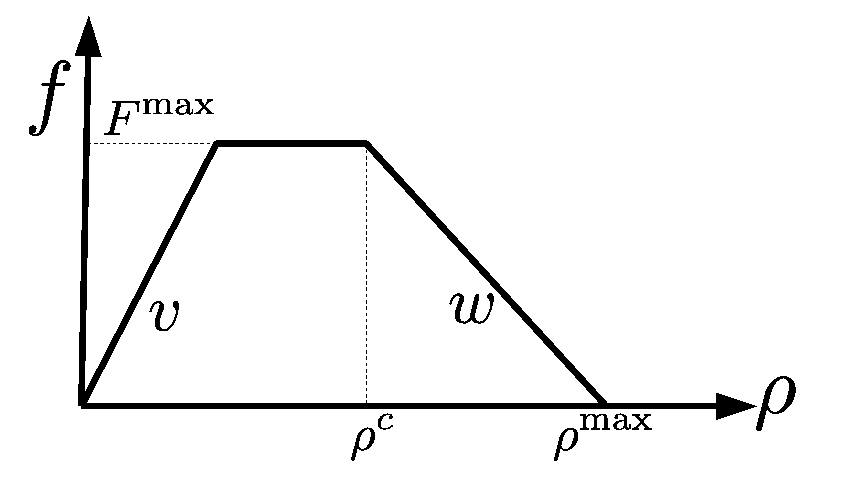
\includegraphics[width=0.4\columnwidth]{figs-gen/fd}
\par\end{centering}

\caption{Fundamental diagram (the name of the flux function in transportation
literature) with free-flow speed $v$, congestion wave speed $w$,
max flux $F^{\max}$, critical density $\density^{c}$, and max density
$\density^{\max}$.\label{fig:Fundamental-diagram-with}}
\end{wrapfigure}%


As control input, an on-ramp $2\link-1\in\links,\link\in\intrange 1{\nlinks}$
at time-step $k\in\intrange 0{\ntime-1}$ has a metering rate $\ramp_{2\link-1}^{\tind}\in\left[0,1\right]$
which limits the flux of vehicles leaving the on-ramp. Intuitively,
the metering rate acts as a fractional decrease in the flow leaving
the on-ramp and entering the mainline freeway. The domain of the metering
control is to force the control to neither impose negative flows nor
send more vehicles than present in a queue. Its mathematical model
is expressed in~\eqref{eq:ramp-eqn}.

For notational simplicity we define the set of densities of links
incident to $\jup{2\link}=\jdown{2\left(\link-1\right)}$ at time-step
$\tind$ as $\juncstate{\jup{2\link}}{\tind}=\left\{ \discrete{2\left(\link-1\right)}{\tind},\discrete{2i-1}{\tind},\discrete{2\link}{\tind}\right\} $. For $k\in\intrange 1{\ntime-1}$,
the mainline density $\discrete{2\link}{\tind}$ using the Godunov
scheme from~\eqref{eq:main-ge} is given by:

\begin{eqnarray}
\syseq_{2\link}^{\tind}(\state,\control)= & \discrete{2\link}{\tind}-\discrete{2\link}{\tind-1} & +\dfrac{\Delta t}{\length_{2\link}}\left(\god_{\jdown{2\link}}\left(\juncstate{\jdown{2\link}}{\tind-1},\ramp_{2\link+1}^{\tind-1}\right)\right)_{2\link}\label{eq:rho-update}\\
&  & -\dfrac{\Delta t}{\length_{2\link}}\left(\god_{\jup{2\link}}\left(\juncstate{\jup{2\link}}{\tind-1},\ramp_{2\link-1}^{\tind-1}\right)\right)_{2\link}\nonumber \\
= & \discrete{2\link}{\tind}-\discrete{2\link}{\tind-1} & +\frac{\Delta t}{\length_{2\link}}\left(\fout{2\link}{\tind-1}-\fin{2\link}{\tind-1}\right)=0
\end{eqnarray}
where we have introduced some substitutions to reduce the notational
burden of this section: $\fout{\link}{\tind}$ is the Godunov flux
at time-step $\tind$ exiting a link $\link$ at the downstream boundary
of the link, and $\fin{\link}{\tind}$ is the Godunov flux entering
the link at the upstream boundary.

We also make the assumption that on-ramps have infinite capacity and
a free-flow velocity $\ffspeed_{2\link-1}=\frac{\length_{2\link-1}}{\Delta t}$
to prevent the ramp congestion from blocking demand from ever entering
the network. Since the on-ramp has no physical length, the length
is chosen arbitrarily and the ``virtual'' velocity chosen above
is chosen to replicate the dynamics in~\cite{Monache2014PdeOde}. We can
then simplify the on-ramp update equation to be:

\begin{eqnarray}
\syseq_{2\link-1}^{\tind}(\state,\control) & = & \discrete{2\link-1}{\tind}-\discrete{2\link-1}{\tind-1}-\frac{\Delta t}{\length_{2\link-1}}\left(\left(\god_{\jup{2\link}}\left(\juncstate{\jup{2\link}}{\tind-1},\ramp_{2\link-1}^{\tind-1}\right)\right)_{2\link-1}-\boundaryDemand{2\link-1}{\tind-1}\right)\label{eq:on-ramp-update}\\
& = & \discrete{2\link-1}{\tind}-\discrete{2\link-1}{\tind-1}-\frac{\Delta t}{\length_{2\link-1}}\left(\fout{2\link-1}{\tind-1}-\boundaryDemand{2\link-1}{\tind-1}\right)=0
\end{eqnarray}
where $\boundaryDemand{2\link-1}{\tind-1}$ is the on-ramp \emph{flux
}demand, and the same notational simplification has been used for
the downstream flux. This formulation results in ``strong'' boundary
conditions at the on-ramps which guarantees all demand enters the network.
Details on weak versus strong boundary conditions can be found in
\cite{Monache2014PdeOde,strub2006weak,work2010traffic}.

The on-ramp model in~\eqref{eq:on-ramp-update} differs from~\cite{Monache2014PdeOde}
in that we model the on-ramp as a discretized PDE with an infinite
critical density, while~\cite{Monache2014PdeOde} models the on-ramp
as an ODE ``buffer''. While both models implement strong boundary
conditions, the discretized PDE model makes the freeway network more
aligned with the PDE network framework presented in this article.


\paragraph{Riemann solver.}

For the ramp metering problem, there are many potential Riemann solvers
that satisfy the properties required in Section~\ref{sub:Network-of-PDE's}.
Following the model of \cite{Monache2014PdeOde}, for each junction $\jup{2\link}$,
we add two modeling decisions:
\begin{enumerate}
\item The flux solution maximizes the outgoing mainline flux $\fin{2\link}{\tind}$.
\item Subject to (1), the flux solution attempts to satisfy $\fout{2\left(\link-1\right)}{\tind}=p_{2(\link-1)}\fout{2\link-1}{\tind}$,
where $p_{2(\link-1)}\in\mathbb{R}_{+}$ is a merging parameter for
junction $\jdown{2\left(\link-1\right)}$. Since (1) allows multiple
flux solutions at the junction, (2) is necessary to obtain a unique
solution.
\end{enumerate}


This leads to the following system of equations that gives the flux
solution of the Riemann solver at time-step $k\in\intrange 1{\ntime-1}$
and junction $\jup{2\link}$ for $\link\in\intrange 1{\nlinks}$:

\begin{eqnarray}
\demand_{2\left(\link-1\right)}^{\tind} & = & \min\left(\ffspeed_{2\left(i-1\right)}\densitydiscrete{2\left(\link-1\right)}{\tind},F_{2\left(\link-1\right)}^{\max}\right)\label{eq:first-ramp}\\
\supply_{2\link}^{\tind} & = & \min\left(\congspeed_{2i}\left(\density_{2i}^{\max}-\densitydiscrete{2\link}{\tind}\right),F_{2i}^{\max}\right)\label{eq:supply}\\
\rampDemand_{2\link-1}^{\tind} & = & \ramp_{2\link-1}^{\tind}\min\left(\frac{\length_{2\link-1}}{\Delta t}\densitydiscrete{2\link-1}{\tind},F_{2i-1}^{\max}\right)\label{eq:ramp-eqn}\\
\fin{2\link}{\tind} & = & \min\left(\splitratio_{2\left(\link-1\right)}^{\tind}\demand_{2\left(\link-1\right)}^{\tind}+\rampDemand_{2\link-1}^{\tind},\supply_{2\link}^{\tind}\right)\label{eq:fin}\\
\fout{2\left(\link-1\right)}{\tind} & = & \begin{cases}
\demand_{2\left(\link-1\right)}^{\tind} & \frac{p_{2(\link-1)}\fin{2\link}{\tind}}{\splitratio_{2\left(\link-1\right)}^{\tind}\left(1+p_{2(\link-1)}\right)}\ge\demand_{2\left(\link-1\right)}^{\tind}\hfill\text{[Case 1]}\\
\frac{\fin{2\link}{\tind}-\rampDemand_{2\link-1}^{\tind}}{\splitratio_{2\left(\link-1\right)}^{\tind}} & \frac{\fin{2\link}{\tind}}{1+p_{2(\link-1)}}\ge\rampDemand_{2\link-1}^{\tind}\hfill\text{[Case 2}]\\
\frac{p_{2(\link-1)}\fin{2\link}{\tind}}{\left(1+p_{2(\link-1)}\right)\splitratio_{2\left(\link-1\right)}^{\tind}} & \text{otherwise}\hfill[\text{Case 3]}
\end{cases}\label{eq:merge}\\
\fout{2\link-1}{\tind} & = & \fin{2\link}{\tind}-\splitratio_{2\left(\link-1\right)}^{\tind}\fout{2\left(\link-1\right)}{\tind}\label{eq:last-ramp}
\end{eqnarray}
where, for notational simplicity, at the edges of of the range for
$\link$, any undefined state values (e.g. $\densitydiscrete 0{\tind}$)
are assumed to be zero by convention. 

For $\tind=0$, the update equation is given by a pre-specified initial
condition, as in~\eqref{eq:init-ge}. Note that the equations can
be solved sequentially via forward substitution. Also, we do not include
the flux result for off-ramps explicitly here since its value has no
bearing on further calculations, and we will henceforth ignore its
calculation. To demonstrate that indeed the flux solution satisfies
the flux conservation property, the off-ramp flux is trivially determined
to be $\splitratio_{2\left(\link-1\right)}^{\tind}\fout{2\left(\link-1\right)}{\tind}$.



Equations~\eqref{eq:first-ramp}
and~\eqref{eq:ramp-eqn} determine the maximum flux that can exit
link $2(\link-1)$ and link $2\link-1$ respectively. Equation~\eqref{eq:supply}
gives the maximum flux allowed into link $2\link$. The actual flux
into link $2\link$, shown in~\eqref{eq:fin}, is given as the minimum
of the ``demand'' from upstream links and ``supply'' of the downstream
link. See~\cite{Monache2014PdeOde} for more details on the model for this
equation. The flux out of link $2(\link-1)$ is split into three cases
in~\eqref{eq:merge}. The solutions are depicted in Fig.~\ref{fig:Godunov-junction-flux},
which demonstrates how the flux solution depends upon the respective
demands and the merging parameter $p_{2\left(\link-1\right)}$. Finally,
Equation~\eqref{eq:last-ramp} gives the flux out of the on-ramp $2\link-1$,
which is the difference between the flux into link $2\link$ and the
flux out of link $2\left(\link-1\right)$ the remains on the mainline.
\begin{figure}
\subfloat[Case 1: Priority violated due to limited upstream mainline demand
entering downstream mainline.]{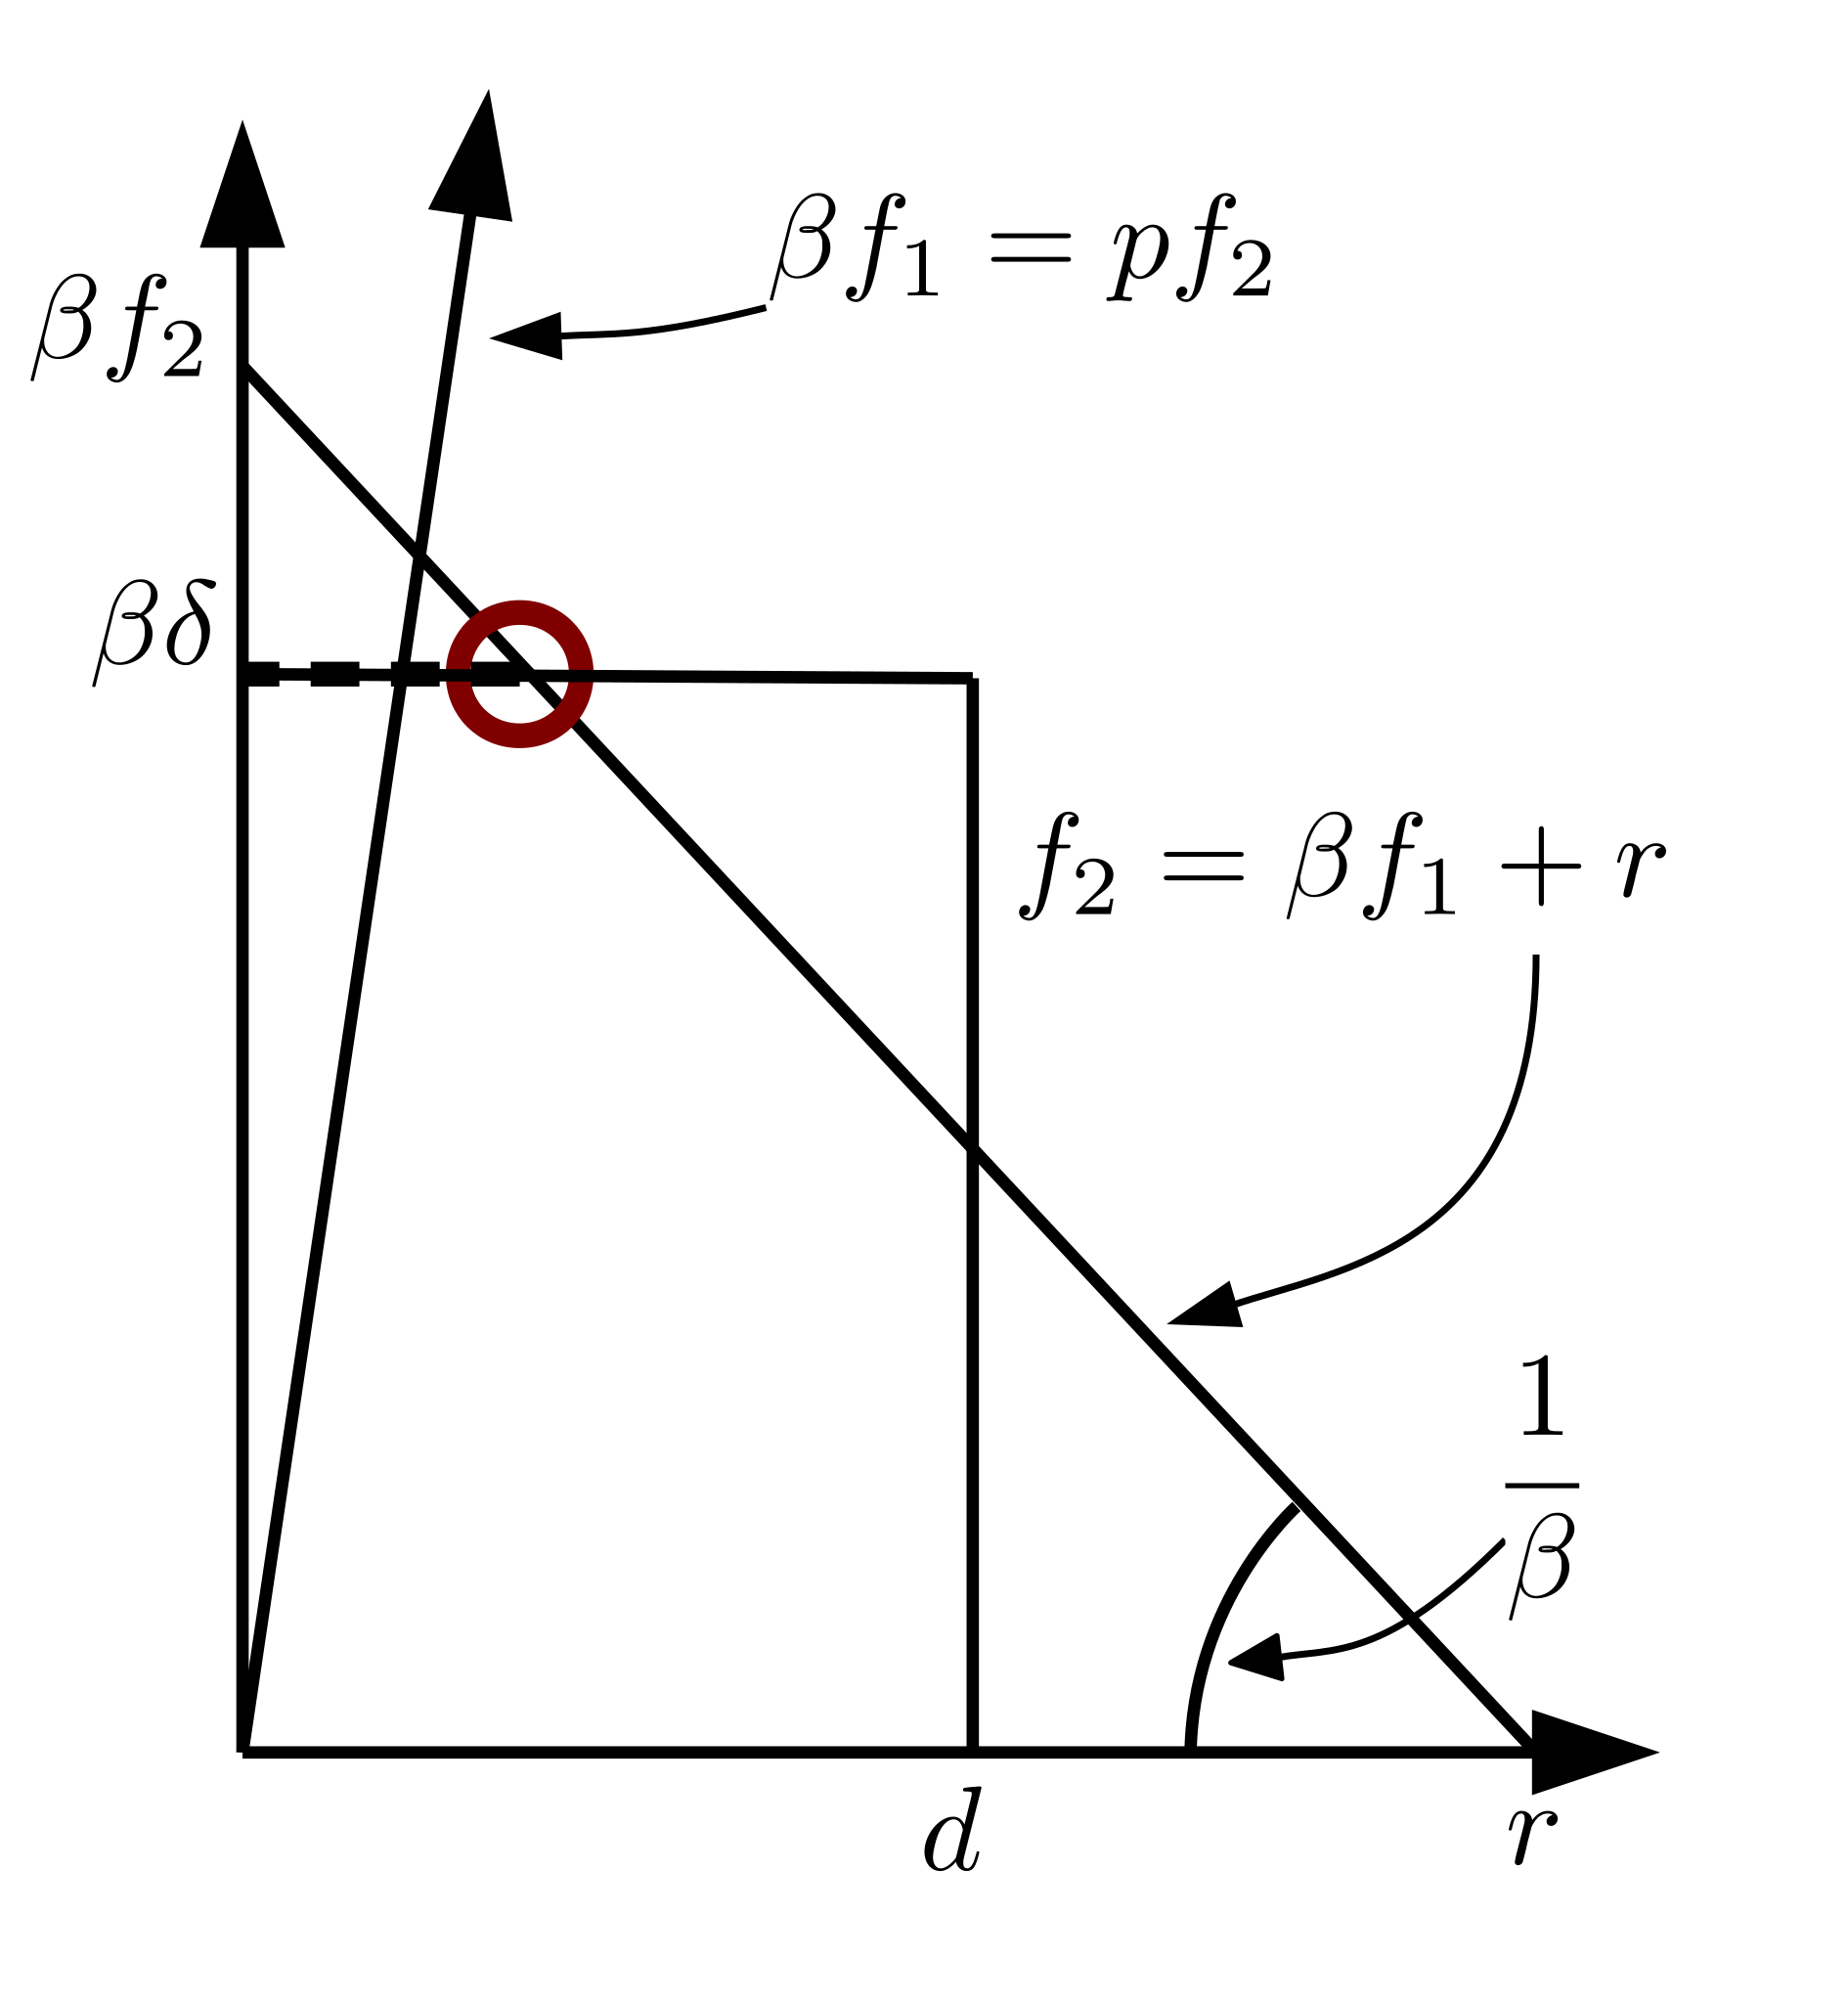
\includegraphics[width=0.3\columnwidth]{figs-gen/flux-sln-1}

}\hfill{}\subfloat[Case 2: Priority violated due to limited on-ramp demand entering downstream
mainline.]{\includegraphics[width=0.3\columnwidth]{figs-gen/flux-sln-2-slim}

}\hfill{}\subfloat[Case 3: Priority rule satisfied due to sufficient demand from both
mainline and on-ramp.]{\includegraphics[width=0.3\columnwidth]{figs-gen/flux-sln-3-slim}

}

\caption{Godunov junction flux solution for ramp metering model at junction
$\jup{2\link}$. The rectangular region represents the feasible flux
values for $\splitratio_{2\left(\link-1\right)}\fout{2\left(\link-1\right)}{}$
and $\fout{2\link-1}{}$ as determined by the upstream demand, while
the line with slope\label{fig:Godunov-junction-flux} $\frac{1}{\splitratio_{2\left(\link-1\right)}}$
represents feasible flux values as determined by mass balance. The
$\splitratio_{2\left(\link-1\right)}\fout{2\left(\link-1\right)}{}$
term accounts for only the flux out of link $2\left(\link-1\right)$
that stays on the mainline. The flux solution, represented by the
red circle, is the point on the feasible region that minimizes the
distance from the priority line $\splitratio_{2\left(\link-1\right)}\fout{2\left(\link-1\right)}{}=p_{2(\link-1)}\fout{2\link-1}{}$.}
\end{figure}


For $\tind=0$, the update equation is given by a pre-specified initial
condition, as in~\eqref{eq:init-ge}. Note that the equations can
be solved sequentially via forward substitution. Also, we do not include
the flux result for off-ramps explicitly here since its value has no
bearing on further calculations, and we will henceforth ignore its
calculation. To demonstrate that indeed the flux solution satisfies
the flux conservation property, the off-ramp flux is trivially determined
to be $\splitratio_{2\left(\link-1\right)}^{\tind}\fout{2\left(\link-1\right)}{\tind}$.


\subsection{Formulation of the Optimal Control Problem}


\paragraph{Optimal coordinated ramp-metering.}

Including the initial conditions as specified in~\eqref{eq:init-ge}
with~\eqref{eq:rho-update} and~\eqref{eq:on-ramp-update} gives
a complete description of the system $\sys\left(\state,\control\right)=0$,
$\state\in\mathbb{R}^{2\nlinks}$, $\control\in\mathbb{R}$, where:

\begin{eqnarray*}
\state_{2\nlinks\tind+\link}\defeq & \densitydiscrete{\link}{\tind} & 1\le i\le2\nlinks,0\le k\le T-1\\
\control_{\nlinks\tind+\link}\defeq & \ramp_{2\link}^{\tind} & 1\le i\le\nlinks,0\le k\le T-1
\end{eqnarray*}


The objective of the control is to minimize the \emph{total travel
time }on the network, expressed by the cost function $\cost$:

\[
\cost\left(\state,\control\right)=\Delta t\sum_{k=1}^{T}\sum_{i=1}^{2\nlinks}L_{i}\densitydiscrete{\link}{\tind}.
\]


The optimal coordinated ramp-metering problem can be formulated as
an optimization problem with PDE-network constraints:

\begin{eqnarray}
\min_{\control} & \cost\left(\state,\control\right)\label{eq:full}\\
\text{subject to:} & \sys\left(\state,\control\right) & =0\nonumber \\
& 0\le\convar\le1 & \forall\convar\in\control  \label{eq:box}
\end{eqnarray}

Standard methods exist for the handling of geometric constraints on $\mathbf{u}$ in descent methods (such as box constraints in Equation~\eqref{eq:box}), such as projection methods~\cite{Apice2010Modeling} and barrier methods~\cite{Fiacco1990Nonlinear,Boyd2010,Bayen2006}.

%Since the adjoint method in Section~\ref{sec:Adjoint-method} only
%deals with equality constraints, we add barrier penalties to the cost
%function~\cite{Boyd2010,Bayen2006}:

% \begin{equation}
% \tilde{\cost}\left(\state,\control,\epsilon\right)=\cost\left(\state,\control\right)-\barrierTerm\sum_{\convar\in\control}\log\left(\left(1-\convar\right)\left(\convar-0\right)\right)\label{eq:full-tilde}.
% \end{equation}


% As $\barrierTerm\in\mathbb{R}^{+}$ tends to zero, the solution to~\eqref{eq:full-tilde}
% will approach the solution to the original problem~\eqref{eq:full}.
% Thus we can solve~\eqref{eq:full} by iteratively solving the augmented
% problem:

% \begin{eqnarray}
% \min_{\control} & \tilde{\cost}\left(\state,\control,\epsilon\right)\label{eq:full-1}\\
% \text{subject to:} & \sys\left(\state,\control\right) & =0\nonumber 
% \end{eqnarray}
% with decreasing values of $\barrierTerm$. As a result, $\tilde{\cost}$
% will approach $\cost$ as the number of iterations increases.


\paragraph{Applying the adjoint method.}

To use the adjoint method as described in Section~\ref{sec:Adjoint-method},
we need to compute the partial derivative matrices $\Hx$, $\Hu$,
$\tilde{C}_{\state}$ and $\tilde{C}_{\control}$. Computing the partial
derivatives with respect to the cost function is straight forward:

\begin{eqnarray*}
\pfrac{\tilde{\cost}}{\discrete{\link}{\tind}}= & \Delta tL_{i} & 1\le i\le2\nlinks,0\le k\le T-1\\
\pfrac{\tilde{\cost}}{\ramp_{2\link}^{\tind}}= & \barrierTerm\left(\frac{1}{1-\ramp_{2\link}^{\tind}}-\frac{1}{\ramp_{2\link}^{\tind}}\right) & 1\le i\le\nlinks,0\le k\le T-1
\end{eqnarray*}


To compute the partial derivatives of $\sys$, we follow the procedure
in Section~\ref{par:Calculating-the-gradient}. For an upstream junction
$\jup{2\link}\in\jns$ and time-step $k\in\intrange 1{\ntime-1}$,
we only need to compute the partial derivatives of the flux solver
$\god_{\jup{2\link}}\left(\juncstate{\jup{2\link}}{\tind},\ramp_{2\link-1}^{\tind}\right)_{\text{}}$
with respect to the adjacent state variables $\juncstate{\jn_{\link}}{\tind}$
and ramp metering control $\ramp_{\link}^{\tind}$. We calculate the
partial derivatives of the functions in~\eqref{eq:first-ramp}-\eqref{eq:last-ramp}
with respect to either a state or control variable$s\in\state\cup\control$:

\begin{eqnarray*}
\pfrac{\demand_{2\left(\link-1\right)}^{\tind}}s & = & \begin{cases}
\ffspeed_{2\left(i-1\right)} & s=\densitydiscrete{2\left(\link-1\right)}{\tind},\ffspeed_{i}\densitydiscrete{2\left(\link-1\right)}{\tind}\le F_{2\left(i-1\right)}^{\max}\\
0 & \text{otherwise}
\end{cases}\\
\pfrac{\supply_{2\link}^{\tind}}s & = & \begin{cases}
-\congspeed_{2i} & s=\densitydiscrete{2\link}{\tind},\congspeed_{2i}\left(\density_{2i}^{\max}-\densitydiscrete{2\link}{\tind}\right)\le F_{2i}^{\max}\\
0 & \text{otherwise}
\end{cases}\\
\pfrac ds & = & \begin{cases}
\ramp_{2\link-1}^{\tind} & s=\densitydiscrete{2\link-1}{\tind},\densitydiscrete{2\link-1}{\tind}\le F_{2\link-1}^{\max}\\
\min\left(\densitydiscrete{2\link-1}{\tind},F_{2i-1}^{\max}\right) & s=\ramp_{2\link-1}^{\tind}\\
0 & \text{otherwise}
\end{cases}\\
\pfrac{}s\fin{2\link}{\tind} & = & \begin{cases}
\splitratio_{2\left(\link-1\right)}^{\tind}\pfrac{\demand_{2\left(\link-1\right)}^{\tind}}s+\pfrac{\rampDemand_{2\left(\link-1\right)}^{\tind}}s & \splitratio_{2\left(\link-1\right)}^{\tind}\demand_{2\left(\link-1\right)}^{\tind}+\rampDemand_{2\link-1}^{\tind}\le\supply_{2\link}^{\tind}\\
\pfrac{\supply_{2\link}^{\tind}}s & \text{otherwise}
\end{cases}\\
\pfrac{}s\fout{2\left(\link-1\right)}{} & = & \begin{cases}
\pfrac{\demand_{2\left(\link-1\right)}^{\tind}}s & \frac{\fin{2\link}{\tind}p_{2(\link-1)}}{1+p_{2(\link-1)}}\ge\frac{\demand_{2\left(\link-1\right)}^{\tind}}{\splitratio_{2\left(\link-1\right)}^{\tind}}\\
\frac{1}{\splitratio_{2\left(\link-1\right)}^{\tind}}\left(\pfrac{}s\fin{2\link}{\tind}-\pfrac{\rampDemand_{2\link-1}^{\tind}}s\right) & \frac{\fin{2\link}{\tind}}{1+p_{2(\link-1)}}\ge\rampDemand_{2\left(\link-1\right)}^{\tind}\\
\frac{p_{2(\link-1)}}{\splitratio_{2\left(\link-1\right)}^{\tind}\left(1+p_{2(\link-1)}\right)}\pfrac{}s\fin{2\link}{\tind} & \text{otherwise}
\end{cases}\\
\pfrac{}s\fout{2\link-1}{} & = & \pfrac{}s\fin{2\link}{\tind}-\splitratio_{2\left(\link-1\right)}^{\tind}\pfrac{}s\fout{2\left(\link-1\right)}{}
\end{eqnarray*}


These expressions fully quantify the partial derivative values needed
in~\eqref{eq:dhdugod} and~\eqref{eqdhdvgod}. Thus we can construct
the $\Hx$ and $\Hu$ matrices. With these matrices and $\Jx$ and
$\Ju$, we can solve for the adjoint variable $\lambda\in\mathbb{R}^{2\nlinks\ntime}$
in~\eqref{eq:adjoint} and substitute its value into~\eqref{eq:adjoint-grad}
to obtain the gradient of the cost function $\cost$ with respect
to the control parameter $\control$.

%!TEX root = restart.tex
\section{Numerical Results for Model Predictive Control Implementations\label{sec:Numerical-results-for}}

To demonstrate the effectiveness of using the adjoint ramp metering
method to compute gradients, we implemented the algorithm on practical scenarios with field experimental data.
The algorithm can then be used as a gradient computation subroutine
inside any descent-method optimization solver that takes advantage
of first-order gradient information. Our implementation makes use
of the open-source \emph{IpOpt} solver~\cite{Andreas2005}, an interior point, nonlinear program optimizer. To serve
as comparisons, two other case scenarios were run:
\begin{enumerate}
\item No control: the metering rate is set to 1 on all on-ramps at all times.
\item Alinea~\cite{Papageorgiou1991Alinea}: a well-adopted, feedback-based ramp metering
algorithm commonly used in the practitioner's community. Alinea is computationally efficient and decentralized,
making it a popular choice for large networks, but does not take estimated
boundary flow data as input. Since Alinea has a number of tuning parameters,
we perform a \emph{modified} grid-search technique over the different
parameters that scales linearly with the number of on-ramps, and select
the best-performing parameters, in order to be fair to this framework. A \emph{full} grid-search approach
scales exponentially with the number of on-ramps, rendering it infeasible
for moderate-size freeway networks.
\end{enumerate}
All simulations were run on a 2012 commercial laptop with 8 GB of RAM and a dual-core 1.8 GHz Intel Core i5 processor.

\begin{note} To demonstrate the reduced running time associated with the adjoint approach, we also implemented a gradient descent using a finite differences approach similar to~\cite{Frejo2011,Ramon2013}, which requires an $O(\ntime^2\nlinks\ncontrols)$ computation for each step in gradient descent, but it proved to be computationally infeasible for even small, synthetic
networks. Running ramp metering on even a network of 4 links over
6 time-steps for 5 gradient steps took well over 4 minutes,
rendering the method useless for real-time applications. The comparison
of running times of finite differences versus the adjoint method is given in
Fig.~\ref{fig:Running-time-of}. Due to the impractically large running times associated with finite differences, we do not consider the finite differences in further results, which only becomes worse as the problem scales to larger networks and time horizons.
\end{note}
\begin{figure}
\begin{centering}
\includegraphics[width=0.5\columnwidth]{images/itergrad}
\par\end{centering}

\caption{Running time of ramp metering algorithm using IpOpt with and without gradient information.
Network consists of 4 links and 6 time-steps with synthetic boundary
flux data. The method using gradient information via the adjoint
method converged well before the completion of the \textit{first} step of the finite differences descent method.
\label{fig:Running-time-of}}
\end{figure}



\subsection{Implementation of I15S in San Diego\label{sub:Network}}

As input into the optimization problem, we constructed a model of
a 19.4 mile stretch of the I15 South freeway in San Diego,
California between San Marcos and Mira Mesa. The network has $\nlinks=125$ links, and $\ncontrols=9$ on-ramps,
with boundary data specified for $\ntime=1800$ time-steps,
for a time horizon of 120 minutes given $\Delta t=$4 seconds.
The network is shown in Fig.~\ref{fig:Model-of-section}.
\begin{figure}
\begin{centering}
\includegraphics[width=0.7\columnwidth]{images/map}
\par\end{centering}
\caption{Model of section of I15 South in San Diego, California. The freeway
section spanning 19.4 miles was split into 125 links with 9 on-ramps.\label{fig:Model-of-section}}
\end{figure}


Link length data was obtained using the Scenario Editor software developed
as part of the \textit{Connected Corridors} project, a collaboration between
UC Berkeley and PATH research institute in Berkeley, California.
Fundamental diagram parameters, split ratios, and boundary data were
also obtained using calibration techniques developed by Connected
Corridors. Densities resulting in free-flow speeds were chosen as
initial conditions on the mainline and on-ramps. The data used in calibration
was taken from PeMS sensor data~\cite{Chen2003} during a morning rush hour period,
scaled to generate congested conditions. The input data was chosen
to demonstrate the effectiveness of the adjoint ramp metering method
in a real-world setting. A profile of the mainline and on-ramps during
a forward-simulation of the network is shown in Fig.~\ref{fig:Density-and-queue}
under the described boundary conditions.
\begin{figure}
\subfloat[Density profile. The units are the ratio of a link's vehicle density
to a link's jam density.\label{fig:Density-profile.}]{\includegraphics[width=0.45\columnwidth]{images/ncdensity}
								
}\hfill{}\subfloat[On-ramp queue profile in units of vehicles.\label{fig:Density-profile.-2}]{\includegraphics[width=0.45\columnwidth]{images/ncqueue}
										
}
								
\caption{Density and queue profile of no-control freeway simulation. In the
	first 80 minutes, congestion pockets form on the freeway and queues
	form on the on-ramps, then eventually clear out before 120 minutes.\label{fig:Density-and-queue}}
\end{figure}
						
						
						
\subsection{Finite-Horizon Optimal Control\label{sub:Finite-horizon-optimal-control}}
						
						
\paragraph{Experimental Setup.}
						
The adjoint ramp metering algorithm is compared to the reactive Alinea
scheme, for which we assume that perfect boundary conditions and initial conditions
are available. The metric we use to compare the different strategies is \emph{reduced-congestion} percentage, $\bar{c} \in \left(-\infty,100\right]$, which we define as:
\[
\bar{c} = 100 \left(1 - \frac{c_\text{c}}{c_{\text{nc}}}\right)
\]where $c_\text{c}, c_{\text{nc}} \in \mathbb{R}_+$ are the \emph{congestion} resulting from the \emph{control} and \emph{no-control} scenarios, respectively. We use the metric for congestion as defined in~\cite{Skabardonis2003}; for a given section of road $S$ and time horizon $T$, the congestion is given as
\[
c\left(S,T\right) = \sum_{\left(s\in S, \tau\in T\right)} \max \left[\text{TTT}\left(s,\tau\right) - \frac{\text{VMT}\left(s, \tau\right)}{v_s}, 0\right]
\] where $v_s$ is the free-flow velocity, $\text{VMT}$ is total vehicle miles traveled, and $\text{TTT}$ is total travel time over the link $s$ and time-step $\tau$. Since it is infeasible to compute the global optimum for all cases, a reduced congestion of 100\% serves as an upper bound on the possible amount of improvement.

\paragraph{Results.}
						
\begin{figure}
\subfloat[Density difference profile in units of \emph{change in density} from the control scenario to the no control scenario over the jam density of the link.\label{fig:long-sim-density}]
{
\includegraphics[width=0.45\columnwidth]{images/densdiff}
}
\hfill{}
\subfloat[Queue difference profile in units of vehicles.\label{fig:long-sim-queue}]
{
\includegraphics[width=0.45\columnwidth]{images/queuediff}										
}
\caption{Profile differences for mainline densities and on-ramp queues. Evidenced
	by the mainly negative differences in the mainline densities and the
	mainly positive differences in the on-ramp queue lengths, the adjoint
	ramp metering algorithm effectively limits on-ramp flows in order to
	reduce mainly congestion. \textit{View in color.}\label{fig:long-sim}}
\end{figure}
						
						
Fig.~\ref{fig:long-sim} shows a difference profile for both density and queue lengths between the
no control simulation and the simulation applying the ramp metering
policy generated from the adjoint method. Negative differences in
Figs.~\ref{fig:long-sim-density} and~\ref{fig:long-sim-queue}
indicate where the adjoint method resulted in fewer vehicles for the
specific link and time-step. The adjoint method was successful in
appropriately deciding which ramps should be metered in order to improve
throughput for the mainline.

\begin{figure}
\centering
	\includegraphics[width=0.45\columnwidth]{images/longsim}
	\caption{Reduced congestion versus simulation time for freeway network. The results
		indicate that the algorithm can run with performance better than Alinea
		if given an update time of less than a minute.}
		\label{fig:running-time}
\end{figure}
								
Running time analysis shows that the adjoint method can produce beneficial
results in real-time applications. Fig.~\ref{fig:running-time} details the improvement of the adjoint method as a function of the overall running time of the algorithm. After just a few gradient steps, the
adjoint method outperforms the Alinea method. Given that the time
horizon of two hours is longer than the period of time one can expect
reasonably accurate boundary flow estimates, more practical simulations
with shorter time horizons should permit more gradient steps in a
real-time setting.
								
While the adjoint method leads to queues with a considerable number of cars in some on-ramps, this can be addressed by introducing barrier terms into the cost function that limit the
maximum queue length. The Alinea method tested for the I15 network
had no prescribed maximum queue lengths as well, but was not able
to produce significant improvements in total travel time reduction, while the adjoint method was
more successful.
								
								
\subsection{Model Predictive Control\label{sub:Model-predictive-control}}
								
To study the performance of the algorithm under noisy input data,
we embed both our adjoint ramp metering algorithm and the Alinea algorithm
inside of a \emph{model predictive control }(MPC) loop.
								
								
\paragraph{Experimental Setup.}
								
The MPC loop begins at a time $t$ by estimating the initial conditions
of the traffic on the freeway network and the predicted boundary fluxes
over a certain time horizon $T_{h}$. These values are noisy, as exact
estimation of these parameters is not possible on real freeway networks.
The estimated conditions are then passed to the ramp metering algorithm
to compute an optimal control policy over the $T_{h}$ time period.
The system is then forward-simulated over an update period of $T_{u}\le T_{h}$,
using the exact initial conditions and boundary conditions, as opposed
to the noisy data used to compute control parameters. The state of
the system and boundary conditions at $t+T_{u}$ are then estimated
(with noise) and the process is repeated.
								
A non-negative\emph{ noise factor}, $\noiseFactor \in \R_+$, is used to study how the adjoint
method and Alinea perform as the quality of estimated data decreases. If $\discrete{}{}$ is the actual density for a cell and time-step, then the density $\bar{\discrete{}{}}$ passed to the control schemes is given by:
\[
\bar{\discrete{}{}}=\discrete{}{}\cdot \left(1+\noiseFactor\cdot R\right)
\]
where $R$ is a uniformly distributed random variable with mean $0$
and domain $\left[-0.5,0.5\right]$. The noise factor was applied
to both initial and boundary conditions.
								
Two different experiments were conducted:
\begin{enumerate}
	\item \textbf{Real-time I15 South}: MPC is run for the I15 South network
	with $T_{h}=80$ minutes and $T_{u}=26$ minutes. A noise factor of
	2\% was chosen for the initial and boundary conditions. The number
	of iterations was chosen in order to ensure that each MPC iteration
	finished in the predetermined update time $T_{u}$.
	\item \textbf{Noise Robustness}: MPC is for over a synthetic network with
	length 12 miles and boundary conditions over 75 minutes. The experiments
	are run over a profile of noise factors between 1\% and 8000\%.
\end{enumerate}
								
\paragraph{Results.}
								
% \subparagraph{Real-Time I15 South.}
\textbf{Real-Time I15 South.} The results are summarized in Fig.~\ref{fig:MPC-performance-on}.
The adjoint method applied once to the entire horizon with perfect
boundary and initial condition information serves as a baseline performance
for the other simulations, which had noisy input data and limited
knowledge of predicted boundary conditions. The adjoint method still
performs well under the more realistic conditions of the MPC loop
with noise, resulting in 2\% reduced congestion or 40 car-hours in relation to no control, as compared to the 3\% reduced (60 car-hours) congestion achieved by the adjoint method with no noise and full time horizon ($T_h=T$). In comparison, the Alinea method was only able to achieve 1.5\% reduced congestion (30 car-hours) for both the noisy and no-noise scenarios. The results indicate
that, under a realistic assumption of a 2\% noise factor in the sensor
information, the algorithm's ability to consider boundary conditions results in an improvement upon strictly reactive policies,
such as Alinea.
								
\begin{figure}
	\subfloat[Reduced congestion.\label{fig:MPC-performance-on}]{\includegraphics[width=0.45\columnwidth]{images/longmpc}
		}\hfill{}\subfloat[Reduced congestion with increasing sensor noise for network with synthetic data.\label{fig:Ramp-metering-performance-1}]{\includegraphics[width=0.45\columnwidth]{images/noiseplot}
	}
	\caption{Summary of model predictive control simulations. The results indicate that the adjoint method has superior performance for moderate noise levels on the initial and boundary conditions.}
\end{figure}

% \subparagraph{Robustness to Noise.}																
\textbf{Robustness to Noise.} Simulation results on the synthetic network with varying levels of
noise are shown in Fig.~\ref{fig:Ramp-metering-performance-1}.
The adjoint method is able to outperform the Alinea method when the
noise level is less than 80\%, a reasonable assumption for data provided
by well-maintained loop detectors. As the initial and boundary condition
data deteriorates, the adjoint method becomes useless. Since Alinea
does not rely on boundary data, it is able to produce improvements,
even with severely noisy data. The results indicate that the adjoint
method will outperform Alinea under reasonable noise levels in the
sensor data.

%!TEX root =restart.tex
\section{Conclusions\label{sec:Conclusions}}

This article has detailed a simple framework for finite-horizon optimal control 
methods on a network of scalar conservation laws derived from first 
discretizing the network via the Godunov method, then applying the discrete 
adjoint to this system. To tailor the framework to a specific application, one 
need only provide the partial derivatives of the Riemann solver at a network 
junction as well as the partial derivatives of the objective. Furthermore, we 
show that for this class of problems, the sparsity pattern allows the problem 
to be implemented with only linear memory and linear computational complexity 
with respect to the number of state and control parameters. We demonstrate the 
scalability of the approach by implementing a coordinated ramp metering 
algorithm using the adjoint method and applying the algorithm to the I-15 South 
freeway in California. The algorithm runs in a fraction of real-time 
and produces significant improvements over existing algorithms. The ramp 
metering algorithm has been fully implemented within Connected 
Corridors~\cite{CC} system, a project by UC Berkeley and PATH for integrated 
corridor management, as a component of the traffic simulator module. Future 
work includes investigating decentralized, coordinated control schemes over physical 
networks via the adjoint method to allow traffic control strategies to scale to 
regional-scale networks.

\section{Acknowledgments}\label{sec:ack}

The authors have been supported by the California Department of Transportation
under the Connected Corridors program, CAREER grant CNS-0845076 under the
project 'Lagrangian Sensing in Large Scale Cyber-Physical Infrastructure
Systems', the European Research Council under the European Union's Seventh Framework Program (FP/2007-2013) / ERC Grant Agreement n. 257661, the INRIA associated team 'Optimal REroute Strategies for Traffic managEment' and the France-Berkeley Fund under the project 'Optimal Traffic Flow Management with GPS Enabled Smartphones'.
% \bibliographystyle{plain}
% \bibliography{AdjointPaper}   % name your BibTeX data base
% \printbibliography
\bibliographystyle{spmpsci}
\bibliography{AdjointPaper,Remote}

\section*{Nomenclature}

\begin{longtable}{|c|c|c|}
	\hline 
	Variable  & Space  & Meaning\tabularnewline
	\hline 
	\hline 
	$t$  & $\mathbb{R}_{+}$  & time\tabularnewline
	\hline 
	$x$  & $\mathbb{R}$  & space\tabularnewline
	\hline 
	$\nlinks$  & $\mathbb{N}$  & Number of links\tabularnewline
	\hline 
	$\jns$  &  & Set of junctions\tabularnewline
	\hline 
	$\links=\left[1,\nlinks\right]$  & $\mathbb{N}^{N}$  & Set of links\tabularnewline
	\hline 
	$L_{\link}$  & $\mathbb{R}_{+}$  & Length of link $\link\in\links$\tabularnewline
	\hline 
	$\cvar_{i}\left(t,x\right)$  & $\mathbb{R}_{+}\times\left]0,L_{i}\right[\rightarrow\mathbb{R}$  & conserved quantity for link $\link\in\links$ as function of $x$\tabularnewline
	\hline 
	$\initstate$  & $BV\cap L_{\text{loc}}^{1}$  & continuous intialial condition\tabularnewline
	\hline 
	$\dvar_{\link}^{\tind}$  & $\mathbb{R}$  & discrete conserved quantity for link $i$ at time-step $k$\tabularnewline
	\hline 
	$f(\cvar)$  & $f:\mathbb{R}\rightarrow\mathbb{R}$  & flux function\tabularnewline
	\hline 
	$\initstate$  & $\mathbb{R}$  & Riemann data\tabularnewline
	\hline 
	$\cvar^{-}$  & $\mathbb{R}$  & Left state of the Riemann data\tabularnewline
	\hline 
	$\cvar^{+}$  & $\mathbb{R}$  & Right state of the Riemann data\tabularnewline
	\hline 
	$\bar{x}$  & $\mathbb{R}$  & Point of discontinuity in Riemann problem\tabularnewline
	\hline 
	$\ssvar$  & $\mathbb{R}$  & Self-similar solution of the Riemann problem\tabularnewline
	\hline 
	$n_{J}$  & $\mathbb{N}$  & Number of incoming links at a junction J\tabularnewline
	\hline 
	$m_{J}$  & $\mathbb{N}$  & Number of outgoing links at a junction J\tabularnewline
	\hline 
	$\Inc\left(\jn\right)=\tuple{\jlink{\jn}1}{\jlink{\jn}{\ninc_{\jn}}}\subset\links$  &  & Set of incoming links at a junction J\tabularnewline
	\hline 
	$\Out\left(\jn\right)=\tuple{\jlink{\jn}{\ninc_{\jn}+1}}{\jlink{\jn}{\ninc_{\jn}+\nout_{\jn}}}\subset\links$  &  & Set of outgoing links at a junction J\tabularnewline
	\hline 
	$\jup{\link}\in\jns$  &  & Upstream junction for the link $\link\in\links$\tabularnewline
	\hline 
	$\jdown{\link}\in\jns$  &  & Downstream junction for the link $\link\in\links$\tabularnewline
	\hline 
	$\RS$  & $\mathbb{R}^{m+n}\rightarrow\mathbb{R}^{m+n}$  & Riemann Solver\tabularnewline
	\hline 
	$\trace{\cvar}_{\link}$  & $\mathbb{R}^{m+n}$  & Trace for a link $i$ at the junction\tabularnewline
	\hline 
	$\Delta t$  & $\mathbb{R}$  & Time grid size\tabularnewline
	\hline 
	$\Delta x$  & $\mathbb{R}$  & Space grid size\tabularnewline
	\hline 
	$t^{\tind}=k\Delta t$  & $k\in\mathbb{N}$  & Time grid points\tabularnewline
	\hline 
	$t^{\xind}=l\Delta x$  & $l\in\mathbb{Z}$  & Space grid points\tabularnewline
	\hline 
	$\lambda^{\max}$  & $\mathbb{R}$  & Wave speed\tabularnewline
	\hline 
	$\juncstate{\jn}{\tind}$  & $\mathbb{R}^{m_{\jn}+n_{\jn}}$  & state variables at a junction $\jn\in\jns$ at a time-step $\tind$\tabularnewline
	\hline 
	$T$  & $\mathbb{N}$  & Number of time steps\tabularnewline
	\hline 
	$\junctrace{\jn}{}$  & $\mathbb{R}^{m_{\jn}+n_{\jn}}$  & solution of $\RS$ at a junction $\jn\in\jns$ at a time-step $\tind$\tabularnewline
	\hline 
	$\junccon{\jn}{\tind}$  & $\mathbb{R}^{\ncontrols_{\jn}}$  & control variables at a junction $\jn\in\jns$ at a time-step $\tind$\tabularnewline
	\hline 
	$\syseq_{\link}^{\tind}$  & $\mathbb{R}^{\nlinks\ntime}\times\mathbb{R}^{\ncontrols\ntime}$  & update equation\tabularnewline
	\hline 
	$\cost$  & $\mathbb{R}^{\nlinks T}\times\mathbb{R}^{N_{\control}T}$  & cost function\tabularnewline
	\hline 
	$\lambda$  & $\mathbb{R}^{\nlinks\ntime}$  & adjoint variable\tabularnewline
	\hline 
	$D_{\state}$  & $\mathbb{N}$  & maximum junction degree on the network \tabularnewline
	\hline 
	$D_{\control}$  & $\mathbb{N}$  & maximum number of constraints \tabularnewline
	\hline 
	$\splitratio_{2\link}^{\tind}$  & $[0,1]$  & off-ramp split ratio \tabularnewline
	\hline 
	$\boundaryDemand{2\link-1}{\tind}$  &  & flux demand at the boundary of on-ramp $2\link-1$\tabularnewline
	\hline 
	$\barrierTerm$  &  & barrier penalty coefficient \tabularnewline
	\hline 
	$\demand_{2\left(\link-1\right)}$  &  & demand on the link $2(i-1)$ \tabularnewline
	\hline 
	$\rampDemand_{2\link-1}^{\tind}$  &  & demand from on-ramp $2\link-1$\tabularnewline
	\hline 
	$\supply_{2\link}^{\tind}$  &  & supply on the link $2i$ \tabularnewline
	\hline 
	$\ffspeed_{\link}$  & $\mathbb{R}_{+}$ & free flow speed for link $\link$\tabularnewline
	\hline 
	$\congspeed_{\link}$  & {[}0,1{]}  & congestion speed $\link$\tabularnewline
	\hline 
	$p_{2\left(\link-1\right)}$  & {[}0,1{]}  & merging parameter \tabularnewline
	\hline 
\end{longtable}


\end{document}
